\documentclass[11pt,a4paper]{article}
\usepackage[T1]{fontenc}
\usepackage[utf8]{inputenc}
\usepackage{lmodern,microtype}
\usepackage[margin=24mm,headheight=14pt]{geometry}
\usepackage{amsmath,amssymb,amsthm,mathtools}
\usepackage{booktabs,longtable,tabularx,array}
\usepackage{enumitem,xcolor,graphicx,float}
\usepackage{fancyhdr,listings}
\usepackage[hidelinks]{hyperref}
\usepackage{bookmark}
\definecolor{ink}{HTML}{153E63}
\definecolor{pale}{HTML}{F1F5F8}
\definecolor{muted}{HTML}{425466}
\hypersetup{pdftitle={Certified primitives for faster unknot recognition},
 pdfauthor={ProveIt research continuation},pdfsubject={Exact algorithms, normal surfaces, tensor networks, compressed words}}
\pagestyle{fancy}
\fancyhf{}
\fancyhead[L]{\small\color{muted}ProveIt: unknot recognition}
\fancyhead[R]{\small\color{muted}8 October 2026}
\fancyfoot[C]{\thepage}
\setlength{\parskip}{4pt}
\setlength{\parindent}{0pt}
\setlength{\emergencystretch}{2em}
\setcounter{tocdepth}{2}
\setlist{topsep=4pt,itemsep=3pt,parsep=0pt}
\newtheorem{theorem}{Theorem}[section]
\newtheorem{lemma}[theorem]{Lemma}
\newtheorem{proposition}[theorem]{Proposition}
\newtheorem{corollary}[theorem]{Corollary}
\theoremstyle{definition}
\newtheorem{definition}[theorem]{Definition}
\newtheorem{question}[theorem]{Research question}
\theoremstyle{remark}
\newtheorem{remark}[theorem]{Remark}
\newcommand{\Z}{\mathbb Z}
\newcommand{\R}{\mathbb R}
\newcommand{\N}{\mathbb N}
\newcommand{\poly}{\operatorname{poly}}
\newcommand{\bits}{\operatorname{bits}}
\newcommand{\lone}[1]{\left\lVert #1\right\rVert_1}
\newcommand{\code}[1]{\texttt{\small #1}}
\newcommand{\status}[1]{\textsf{#1}}
\newcommand{\baseline}{\texttt{8a95834940cf77cdab1b39571ffc102ca8b6bede}}
\newcolumntype{Y}{>{\raggedright\arraybackslash}X}
\newcolumntype{P}[1]{>{\raggedright\arraybackslash}p{#1}}
\lstset{basicstyle=\ttfamily\footnotesize,breaklines=true,columns=fullflexible,
 keepspaces=true,showstringspaces=false,frame=single,rulecolor=\color{pale},
 backgroundcolor=\color{pale},xleftmargin=5pt,xrightmargin=5pt,
 aboveskip=8pt,belowskip=8pt}
\title{\color{ink}\bfseries Certified primitives for faster\\unknot recognition\\[7pt]
 \large Binary planar tensors, optimal cocycle seeds, and compressed overlap witnesses\\[5pt]
 \normalsize A research continuation toward quasi-polynomial complexity}
\author{ProveIt research continuation\\\small Prepared for Vladimir Reshetnikov with ChatGPT Pro}
\date{8 October 2026}
\begin{document}
\maketitle
\begin{abstract}
We continue the performance program in \emph{ProveIt/Topology/UnknotRecognition}
from an explicitly pinned repository revision. Three exact improvements are
developed, implemented, and tested. First, a two-state planar tensor model
computes the full Jones polynomial with at most $2^w$ frontier states, where
$w$ is the crossing-edge cut width of a certified scan order. A combinatorial
rotation cochain supplies the correct contribution of every smoothed circle,
including diagrams with repeated face walks, loops, and nested circles.
The existing planar separator certificate then gives bit time and space
$\poly(n)2^{O(\sqrt n)}$, removing the logarithmic factor in the exponent
of the repository's faithful equality-partition backend. Exact integer
specialization with balanced-digit recovery and valuation normalization is
also provided. This realizes a known square-root-exponential principle in
the present implementation; it is not a claim of the first such theorem.

Second, for an integral cocycle in a finite triangulation, we minimize the
number of normal discs over all global vertex-potential changes. A sparse
integral min-cost flow gives an optimal potential and a matching certificate
whose equality with the primal objective proves optimality over both real
and integral potentials. The conservative bit bound is
$O(T^3(B+\log(T+1)))$ for $T$ tetrahedra and $B$-bit local heights. Under the
stated geometric hypotheses, an optimum has no nonempty relatively
null-homologous component union; a primitive rank-one class therefore gives
a connected nonseparating seed. This preserves a property already enjoyed by
the initial spanning-tree gauge while reducing its disc count.

Third, an optional compressed cyclic-overlap policy asks for a strict-majority
witness before extending its alignment with at most two exact longest common
prefix queries. It is complete for the existence of a local shortening move
when uncapped, and is much faster on a rigorously specified exponential-word
family. It need not find the best greedy move, and the supplied knot corpus
shows no demonstrated recognition speedup from this policy.

Proofs, independent checks, controlled measurements, negative results,
integration patches, and reproduction scripts accompany the article. None of
these improvements establishes a quasi-polynomial worst-case bound for the
complete maintained recognizer. We formulate the remaining requirements in
terms of compressed geometry, hierarchy resets, state growth, and search
completeness, and give a prioritized research agenda with falsifiable targets.
\end{abstract}
\vspace{5pt}
\noindent\fcolorbox{ink}{pale}{\parbox{0.94\linewidth}{\small
\textbf{Scope of the result.} Theorems in this article certify the stated
primitives. Experimental timings measure the supplied instances on one
environment. A Jones polynomial equal to one remains an inconclusive result
in this implementation. A general quasi-polynomial recognition theorem is
\emph{not} claimed.}}
\clearpage
\tableofcontents
\clearpage
\section{Research objective and evidence boundary}
\label{sec:scope}

The objective is to make exact unknot recognition faster while moving toward
a defensible quasi-polynomial worst-case analysis. That requires a joint
argument about topology, representation size, primitive bit costs, and the
number of primitive calls. Speeding up one operation does not supply the
missing bounds on the other three. The work below therefore treats an
implemented theorem, an observed acceleration, and a proposed global route
as different kinds of evidence.

The baseline is the public ProveIt revision
\begin{center}\small\baseline\end{center}
dated 8 October 2026, 15:40:39 UTC. All code changes in the accompanying patch
are relative to that revision. The target is
\code{Topology/UnknotRecognition/fast}; the older reports and synthesis
documents provide mathematical context and selected independent reference
implementations. No remote repository changes are required to inspect or
reproduce this package.

\subsection{Input size and the asymptotic target}

An input knot diagram has $n$ crossings and a validated planar-diagram
encoding. Arc labels are normalized during validation; their accidental
decimal spelling is not a topological size parameter. We use bit complexity
throughout. Writing a bound as polynomial in $n$ permits the usual
$O(n\log(n+2))$ encoding overhead. For a triangulation, $T$ denotes the number
of tetrahedra and $B$ the bit length of supplied integral cocycle heights.
For a compressed word, the grammar size and the bit length of its represented
length are input parameters; the expanded length can be exponential in them.

For an input encoding of length $N$, quasi-polynomial time means
\[
 \exp\!\left((\log(N+2))^{O(1)}\right).
\]
In particular $N^{C\log N}$ is quasi-polynomial, whereas
$2^{C\sqrt N}$ is a larger asymptotic class. Removing a factor $\log n$ from
an exponent $O(\sqrt n\log n)$ is a real improvement, but it does not reach
the requested target. Conversely, a polynomial operation on a $2^N$-letter
word is efficient only if the polynomial is in the compressed encoding,
not in $2^N$.

Three separate resource notions recur:
\begin{enumerate}
\item \emph{Mathematical input size}: the diagram, triangulation, grammar,
and binary integers specified by the theorem.
\item \emph{Represented intermediate size}: frontier keys, coefficient
bits, grammar nodes, attaching maps, or normal coordinates actually stored.
\item \emph{Charged implementation work}: a documented counter or elapsed
time allowance. A cap on state count is not a byte-memory cap, and a cap on
work does not turn an unfinished search into a negative mathematical answer.
\end{enumerate}

\subsection{What the existing implementation already supplies}

The maintained recognizer is a portfolio. It validates the input, applies
structural and simplification certificates, uses one-sided invariant tests,
and can attempt independently replayed group certificates. Complete exact
fallbacks include the built-in Khovanov calculation and an optional external
normal-surface engine. The previous work already includes separator
certificates, exact faithful Potts evaluation, transfer methods for special
diagram families, compressed group words, accelerated repeated automorphisms,
whole-donor macros, and a complete local compressed substring primitive.

The relevant baseline guarantees are narrower than a complete recognition
bound. A crossing scan with certified edge frontier $O(\sqrt n)$ is already
available. The faithful Potts calculation uses equality partitions, whose
Bell-number state count gives $2^{O(w\log(w+2))}$ for $w$ active boundary
objects. Its universal full-polynomial bound is thus
$\poly(n)2^{O(\sqrt n\log n)}$. The compressed word kernel has polynomial
local bit bounds, but no general bound on discovery steps or accumulated
grammar size follows. The normal-surface adapter can return an exact decision
from its external engine, but it does not yet export an independently replayed
compressed hierarchy with a quasi-polynomial running-time theorem.

This continuation reuses those working parts. It changes the state space of
the full-Jones calculation, optimizes a concrete geometric primitive, and
reduces work spent finding a sufficient compressed overlap. The three routes
share a principle: a compact representation must preserve the information
needed by the next exact operation, and its certificate must describe that
operation's actual conclusion.

\subsection{Relationship to the literature}

The Kauffman state model and its normalization are classical
\cite{kauffman1987}. Ellenberg, Newman, Sawin, and Shi already proved a
polynomial-times-$2^{C\sqrt n}$ time and memory bound for the Kauffman bracket
using controlled tangle boundaries \cite{ellenberg2013}. General planar
Boolean tensor contraction and Jones tensor implementations provide further
context \cite{liuying2023,meichanetzidis2019,laakkonen2026}. Our contribution
here is a self-contained binary model that works with the repository's
existing arbitrary crossing cut order, its exact arithmetic, its input
validation, and its resource semantics. The square-root-exponential exponent
itself is established prior work.

The geometry route is motivated by Lackenby's hierarchy construction
\cite{lackenby2026}. It is necessary to distinguish the 2021 announcement of
a quasi-polynomial unknot-recognition algorithm \cite{oxford2021} from the
particular written argument audited here. Section 9 of the July 2026 preprint
does not specify all primitive running times; its iteration estimate depends
on maximal hierarchy length and maximal pattern-complexity. Section 10
improves the depth control, but the code in this package does not implement
all of that geometric machinery. Thus neither the announcement nor the
preprint is used as a black-box complexity proof for ProveIt's recognizer.

Integral optimization through network matrices is also classical. The
topological use of total unimodularity has substantial precedent, including
optimal homologous cycle algorithms \cite{dey2011}. We claim a precise
local-span optimization, certificate, and geometric preservation argument
for the implemented cocycle-seed family, without asserting literature-wide
priority for network integrality or for connected nonseparating surfaces.

\subsection{A current claim about Jones detection and its audited prerequisites}
\label{sec:jones-status}

The literature check was made on 8 October 2026. Carmi and Cohen's
June 2026 preprint explicitly claims that the Jones polynomial detects the
unknot \cite[Theorem~6.9]{carmicohen2026}. The arXiv record inspected on that
date lists version~1 only and displays no withdrawal notice. This claim
must be acknowledged; it cannot be resolved by repeating older descriptions
of the problem's status. Our theorems and recognition decisions do not assume
the claimed detection theorem.

There is a concrete reason for this independence. The pinned repository
already contains an audit of a prerequisite consequence of that preprint.
Lemma~5.8, combined with the universal realization asserted in
Proposition~5.12 and the threshold in Section~5.1.1, implies a uniform bound
on the degree in $p=x-x^{-1}$ of every ordinary residual twist state:
\[
 \deg_p V\le B_{\rm host}+11+2.
\]
Here the expansion is $V(x)=a(p)+b(p)x$, and the degree means
$\max(\deg a,\deg b)$. This implication precedes the low-order anchor
vanishing used later in Theorem~5.10; it is not restricted to hosts already
known to have trivial Jones polynomial \cite[Sections~5.1--5.6]{carmicohen2026}.

For clarity, the existing witness can be described without any clasp-machine
isotopy. Take the three-crossing host with planar-diagram rows
\[
 (5,1,2,0),\quad(1,4,3,2),\quad(0,3,4,5).
\]
Replace the third row by an odd anti-parallel twist of length $L$, keeping
its exterior ports fixed. Explicitly, the first twist row begins with
$(a_0,b_0)=(0,3)$. At row $i=0,\ldots,L-1$ use
$(a_i,b_i,c_i,d_i)$, where $(c_i,d_i)=(6+2i,7+2i)$ for $i<L-1$,
$(c_{L-1},d_{L-1})=(4,5)$, and
$(a_{i+1},b_{i+1})=(d_i,c_i)$. These are the same fixed-exterior
diagrams used by the baseline audit.

Their knot Jones polynomials, in $t=x^2$, satisfy the audited skein recurrence
\[
 V_1(t)=t+t^3-t^4,\qquad
 V_L(t)=t^2V_{L-2}(t)+t-t^2+t^3-t^4.
\]
Consequently the highest term is $-t^{L+3}$. The identity
$x^m=F_{m-1}(p)+F_m(p)x$, with
\[
 F_m(p)=\sum_{k=0}^{\lfloor(m-1)/2\rfloor}
          \binom{m-k-1}{k}p^{m-2k-1},
\]
shows that the corresponding $b$-polynomial has leading term
$-p^{2L+5}$. All lower $t$-powers contribute smaller $p$-degrees.
Thus the degree is $2L+5$; for the mirror it is $2L+6$.

The host has $B_{\rm host}=3\cdot3+1-1=9$, so the proposed uniform
residual cap is $22$. The baseline's $L=9$ witness has degree $23$.
The present package independently recomputes its complete Jones polynomial
with Regina~7.4.1, and recomputes the formal expansion using the displayed
binomial formula rather than the baseline's coefficient recurrence.
It also checks $L=23$: the degree is $51$, while $L>22$ even satisfies
the long-twist inequality needed by the later descent. The mirror degrees
are $24$ and $52$, respectively. All four polynomial computations agree
coefficient by coefficient with all three tensor arithmetic modes.

The original audit additionally records local oriented-smoothing reductions
and Reidemeister-II anchor cancellations. Our new independent computation
replicates its polynomial obstruction. It neither constructs a nontrivial
knot with Jones polynomial one nor identifies a unique erroneous
clasp-machine step. It shows that the stated universal geometric realization
and uniform residual-degree consequence cannot both apply to these explicit
ordinary twists. Accordingly, a Jones polynomial different from one gives
the usual nontriviality obstruction, whereas identity remains inconclusive
in this implementation. The source and complete raw outputs are
\path{reproduce/audit_regina_jones.py} and
\path{results/regina_jones_20261008.json}.


\subsection{The principal results and their scope}

\begin{table}[H]
\centering\small
\begin{tabularx}{\linewidth}{@{}P{0.20\linewidth}YY@{}}
\toprule
Primitive & Proved improvement & Remaining limitation\\
\midrule
Full Jones polynomial & Binary frontier states; exact
$\poly(n)2^{O(\sqrt n)}$ bit bound with a certified separator order &
Subexponential rather than quasi-polynomial; identity is not accepted as an
unknot certificate by this implementation.\\[4pt]
Cocycle normal seed & Exact minimum disc count within a fixed
vertex-potential family; polynomial binary cost and a short dual certificate &
Restricted family; no incompressibility, genus-minimality, or hierarchy-reset
bound.\\[4pt]
Compressed overlap & A sufficient strict-majority witness followed by at most
two LCP extensions; exact local-existence completeness when uncapped &
May choose a worse greedy move; preceding stages and total search remain
possible bottlenecks.\\
\bottomrule
\end{tabularx}
\caption{Theorem scope. Each result is used only for the conclusion it proves.}
\label{tab:scope}
\end{table}

The paper's algorithmic claims are proved below and checked against independent
oracles where feasible. Those checks increase confidence in the implementation;
finite tests do not establish the asymptotic theorems. Conversely, a correct
proof of an algorithm does not excuse a mismatch between the mathematical
algorithm and the code. The package therefore retains full inputs, exact
outputs, proof traces where available, source hashes, and censored observations.

\section{Exact full Jones computation with binary planar tensors}
\label{sec:tensor}

The extra logarithm in the faithful partition backend comes from remembering
an equality relation among frontier objects. A binary tensor model can instead
remember one orientation bit per frontier edge. The difficulty is the loop
factor: summing the two orientations of a smoothed circle must produce the
Kauffman factor, independently of its shape or nesting. A combinatorial
rotation cochain supplies this information without drawing coordinates or
floating-point angles.

\subsection{A checked rotation cochain}

Assume first that $n>0$. The validated one-component classical diagram gives
a connected four-valent graph cellularly embedded in the sphere. Multiple
edges, loops, and repeated vertices in a face boundary are allowed. Its
$4n$ darts are numbered by crossing and counterclockwise port. Let $\alpha$
reverse an edge and let $\rho$ advance one port at a crossing. The face walks
are the cycles of $\rho\alpha$, in the convention used by the implementation.
There are $F=n+2$ faces and $2n$ edges. A distinguished face $o$ is regarded as
the outer face.

Assign an integer bend $\beta(d)$ to each dart, with
$\beta(\alpha d)=-\beta(d)$. The local corner of a positive face-boundary
walk contributes one quarter turn. We require
\begin{equation}
 \sum_{d\in f}\beta(d)=b_f,\qquad
 b_f=\begin{cases}4-|f|,&f\ne o,\\-4-|o|,&f=o.\end{cases}
 \label{eq:face-bends}
\end{equation}
Thus bounded faces have total turn $4$ and the outer face has total turn
$-4$. The word ``positive'' here denotes the selected permutation convention;
no additional claim that a face lies on the left of its traversal is needed.

The demand sum is zero:
\[
 \sum_f b_f=4(F-1)-4-4n=0.
\]
Root a spanning tree of the dual graph at $o$, and send each subtree's total
demand through its parent edge. Put zero bend on non-tree dual edges. This
constructs an integral antisymmetric solution. The implementation checks
every antisymmetry equation and every face sum after routing; it does not
accept the routing procedure itself as the check.

\begin{lemma}[A polynomial bend envelope]
The routed cochain can be chosen to satisfy
\[
 \max_d|\beta(d)|\leq3(n+1),\qquad
 \sum_{\{d,\alpha d\}}|\beta(d)|\leq3(n+1)^2.
\]
\end{lemma}
\begin{proof}
Every face is nonempty. A positive demand is at most $3$, and only the
$n+1$ bounded faces can have positive demand. Since total demand is zero,
the absolute demand of any set of faces is at most total positive demand,
which is at most $3(n+1)$. The dual spanning tree has $F-1=n+1$ edges.
The routed value on each is a subtree demand sum, giving both bounds.
\end{proof}

No metric embedding is required. In particular, long arithmetic coordinates
from a planar straight-line drawing never enter this calculation.

\subsection{Why every smoothed circle has rotation four}

A smoothing at a crossing joins adjacent ports. Write
$\tau(a,b)=+1$ when $b-a\equiv1\pmod4$ and $\tau(a,b)=-1$ when
$b-a\equiv-1\pmod4$. Traversing a smoothing from incoming port $a$ to
outgoing port $b$ contributes $\tau(a,b)$. An edge traversal contributes
the corresponding signed bend. We must prove that the total is always
$+4$ or $-4$ on an oriented smoothed circle.

\begin{lemma}[Rotation of a smoothing component]
For any choice of all $n$ smoothings, every resulting circle has total
combinatorial rotation $+4$ in one orientation and $-4$ in the other.
\label{lem:rotation}
\end{lemma}
\begin{proof}
Work with abstract face disks rather than assuming that each face boundary
is a simple polygon in the projection graph. This retains the correct local
sectors at a loop or a repeated vertex. A chosen smoothing creates a band
between the two uncapped opposite face sectors. On the boundary of the
region receiving the band, two old $+1$ corners become two $-1$ turns. Its
total boundary rotation decreases by $4$, exactly as its Euler characteristic
decreases by $1$ when a band is attached.

Initially each bounded face disk has rotation $4$ by
\eqref{eq:face-bends}. Consequently every bounded complementary region $R$
of the smoothed circles has total boundary rotation $4\chi(R)$. This
argument permits bands within one region and between distinct regions; it
depends only on the Euler change under a band attachment.

An innermost smoothed circle bounds a disk and therefore has rotation $4$
in its positive boundary direction. Now proceed outward through the nesting
of circles. A bounded complementary region with $h$ holes has
$\chi(R)=1-h$. Each already treated inner boundary contributes $-4$ with
the region's boundary direction. Therefore its outer boundary has rotation
$4(1-h)+4h=4$. This proves the assertion for all circles. Reversing direction
negates every corner turn and bend, giving $-4$.
\end{proof}

This proof addresses precisely the cases that a naive appeal to a polygonal
turning-number picture can overlook: repeated face walks, self-loops, and
nested components. It also explains why assigning a formal loop weight at
an arbitrary frontier connectivity is unnecessary in the binary model.

\subsection{Local tensors and normalization}

Use the Kauffman bracket convention in which a state with $c$ circles has
loop factor $\delta^c$, with
\[
 \delta=-A^2-A^{-2}.
\]
The normalized Jones polynomial divides by one loop factor. Make the formal
substitution
\[
 A=i z^2,\qquad \delta=z^4+z^{-4}.
\]
Factor out one $i$ per crossing. Smoothing $s=0$ then has weight $z^2$,
and smoothing $s=1$ has weight $-z^{-2}$. All remaining arithmetic is in
$\Z[z,z^{-1}]$.

At a crossing let $\varepsilon_j\in\{+1,-1\}$ denote the orientation of
port $j$, positive when pointing out of the crossing. Edge contraction
identifies opposite port signs. A smoothing joins opposite signs, so a
nonzero crossing tensor has exactly two positive signs and two negative
signs: at most six assignments. The pairings are
\[
 \mathcal P_0=\{(0,1),(2,3)\},\qquad
 \mathcal P_1=\{(0,3),(1,2)\}.
\]
For a compatible pair $(a,b)$ the directed corner contribution is
$-\varepsilon_a\tau(a,b)$, because $\varepsilon_a=-1$ means that the
traversal enters at $a$. Absorb an edge bend at the smaller-numbered dart
only. If $E_v(\varepsilon)$ is the sum of the absorbed signed bends at
crossing $v$, the local tensor entry is
\begin{equation}
 T_v(\varepsilon)=
 \sum_{\substack{s\in\{0,1\}\\
           \varepsilon_a=-\varepsilon_b\ ((a,b)\in\mathcal P_s)}}
 (-1)^s z^{\,2-4s+E_v(\varepsilon)
                   -\sum_{(a,b)\in\mathcal P_s}\varepsilon_a\tau(a,b)}.
 \label{eq:local-tensor}
\end{equation}
Each entry has at most two signed monomials. A loop edge at one crossing
enforces its two endpoint signs locally and never creates a frontier edge.

For clarity, the entries before multiplication by $z^{E_v}$ are as follows.
The asymmetry comes from the fixed turning convention; the closed invariant
is independent of it.
\begin{center}
\begin{tabular}{@{}cccccc@{}}
\toprule
$(+,+,-,-)$ & $(+,-,+,-)$ & $(-,+,+,-)$ & $(+,-,-,+)$ & $(-,+,-,+)$ & $(-,-,+,+)$\\
\midrule
$-z^{-2}$ & $0$ & $z^2$ & $z^2$ & $z^4-z^{-4}$ & $-z^{-2}$\\
\bottomrule
\end{tabular}
\end{center}
The upper bound six is deliberately conservative and remains valid when
local cancellations or loop constraints remove assignments.

Let $F_D(z)$ be the contraction of these tensors. Expanding each local
smoothing choice and then each compatible orientation orients every
smoothed circle independently. Lemma~\ref{lem:rotation} makes its two
orientation weights sum to $z^4+z^{-4}$. Therefore
\begin{equation}
 \langle D\rangle\big|_{A=i z^2}=i^nF_D(z).
 \label{eq:bracket-tensor}
\end{equation}
If $w(D)$ is the writhe, the usual oriented normalization gives
\begin{equation}
 V_D(z^{-8})=
 (-1)^{(n-w(D))/2}z^{-6w(D)}
 \frac{F_D(z)}{z^4+z^{-4}}.
 \label{eq:jones-normalization}
\end{equation}
The exponent $(n-w(D))/2$ is integral. The Laurent implementation performs
an exact division with a checked zero remainder, applies the sign and shift,
and checks that every remaining $z$-exponent is divisible by eight. It
publishes the coefficient dictionary in variable $t=z^{-8}$. The empty
crossing diagram is treated explicitly as the one-component unknot.

\begin{proposition}[Conservative output bounds]
For an $n$-crossing knot diagram,
\[
 V_D(t)=\sum_e c_e t^e,\qquad |e|\leq2n,
 \qquad\sum_e|c_e|\leq4^n.
 \label{prop:jones-bounds}
\]
\end{proposition}
\begin{proof}
In the state sum after division by one loop factor, a state contributes a
monomial times $\delta^{c-1}$. There are $2^n$ states and at most $n+1$
circles in a state of a connected $n$-crossing projection. Its coefficient
mass is at most $2^{c-1}\leq2^n$, so the sum has mass at most $4^n$.
The smoothing monomial has $A$-degree between $-n$ and $n$; the loop factor
adds at most $2n$ in absolute degree, and the writhe correction adds at most
$3n$. Thus the normalized $A$-degree is at most $6n$ in absolute value.
The standard knot normalization has integral $t=A^{-4}$ exponents, which
gives the more than sufficient bound $|e|\leq2n$.
\end{proof}

The code also verifies $V_D(1)=1$ and these bounds. These are useful error
checks, not a substitute for the state-sum proof or an independent polynomial
oracle. A wrong polynomial can satisfy all three.

\subsection{Frontier contraction and the square-root bound}

Fix an ordering of the crossings. After a prefix has been processed, let
$\partial S$ be the edges with exactly one processed endpoint. A state is
one bit for each edge of $\partial S$, with the bit referenced to its
canonical dart. The coefficient for that bit assignment is the sum of all
compatible tensor products in the processed part. The update joins the
current crossing to every compatible assignment, forgets closed edges,
and introduces the new frontier edges. It sums equal output assignments.
There is no remembered partition and no assumption that the processed part
is a disk.

Let $w$ be the maximum number of crossing edges in a prefix cut. There are
at most $2^w$ keys and at most six local transitions per incoming key.
Indexing the bits costs only polynomial overhead. At any intermediate stage
the formal exponent envelope is
\begin{equation}
 |e|\leq B_n:=4n+3(n+1)^2.
 \label{eq:tensor-exponents}
\end{equation}
Indeed a crossing contributes a smoothing exponent of absolute value at most
two and two corner turns of total absolute value at most two; the absorbed
bends contribute at most the cochain's total absolute bend. Expanding at
most six assignments and two monomials per crossing bounds the total
coefficient mass of any partial sum by $12^n$. A coefficient therefore has
$O(n)$ bits, and there are $O(n^2)$ possible Laurent exponents per key.

\begin{theorem}[Binary frontier full-Jones bound]
Given a validated $n$-crossing knot diagram and an order of crossing-edge
frontier width $w$, the full Jones polynomial can be computed exactly in
$\poly(n)2^w$ bit time and space. With the repository's checked planar
separator order this becomes
\[
 \poly(n)2^{O(\sqrt n)}.
\]
\label{thm:tensor}
\end{theorem}
\begin{proof}
The invariant of the update is the partial contraction just described;
induction on the prefix proves it. At the end the frontier is empty, so
\eqref{eq:bracket-tensor} and \eqref{eq:jones-normalization} give the result.
The state count and polynomial arithmetic bounds prove the first claim.

For completeness, a bounded-degree planar graph has recursively balanced
separators of size $O(\sqrt m)$ on an $m$-vertex subproblem
\cite{lipton1979}. List each child subproblem before its separator, as in
the maintained constructor. At a
prefix inside a child, a crossing edge leaving the prefix is incident to
one of the ancestor separators or the current leaf. Since degree is four,
the frontier is bounded by four times the sum of the separator sizes on
that recursion path. Balance gives a geometric series
$\sqrt n+\sqrt{\theta n}+\sqrt{\theta^2n}+\cdots=O(\sqrt n)$ for
some fixed $\theta<1$. The maintained separator constructor supplies an
explicit partition hierarchy; its verifier checks separation, balance,
size, the flattened order, and the resulting width. The tensor backend
constructs and checks this witness before relying on its guarantee.
\end{proof}

The implementation can compare this order with an ordinary scan order and
use the narrower one; the certified witness still bounds the chosen width.
An explicit \code{certified=False} call is a useful ordering ablation, but
it has no universal square-root width promise. Supplying a bad order does
not invalidate the invariant, only its performance.

\subsection{Exact specialization and balanced-digit recovery}

Python sparse Laurent dictionaries carry appreciable overhead. We can
evaluate the tensors at one sufficiently large exact integer and reconstruct
the entire final polynomial, retaining the same frontier state count. This
is a coefficient-bounded Kronecker substitution, not a numerical sample used
as probabilistic evidence.

Choose
\[
 k=\max\!\left(1,\left\lceil\frac{2n+2}{8}\right\rceil\right),
 \qquad z=2^k,\qquad x=z^8\geq4\cdot4^n.
\]
For a first implementation, subtract each local tensor's minimum exponent
$g_v$ and contract its integral value. If $g=\sum_v g_v$, the final integer
is $Z=z^{-g}F_D(z)$. Equation~\eqref{eq:jones-normalization} yields
\begin{equation}
 P(x):=x^{2n}V_D(x^{-1})=
 \frac{(-1)^{(n-w)/2}z^{16n+4-6w+g}Z}{z^8+1}.
 \label{eq:integer-jones}
\end{equation}
A negative power of $z$ is moved into the denominator. Exact integer division
must have zero remainder. The polynomial $P$ has degree at most $4n$, and
each coefficient has absolute value at most $4^n<x/2$.

\begin{lemma}[Balanced recovery]
An integer of the form $P(x)=\sum_{j=0}^{4n}a_jx^j$, with
$|a_j|<x/2$, determines all the $a_j$ uniquely. Iteratively choose the
residue in $[-x/2,x/2)$ and divide the remaining difference by $x$.
\end{lemma}
\begin{proof}
The constant coefficient is the unique allowed representative of the
integer modulo $x$. Subtracting it and dividing by $x$ leaves the same
problem with one fewer coefficient. Induction proves uniqueness and the
algorithm. The recovered coefficient at index $j$ is the coefficient of
$t^{2n-j}$ in $V_D(t)$.
\end{proof}

The intermediate specialized tensor values need not encode their formal
Laurent polynomials injectively. Distinct partial polynomials can specialize
to the same value, and a nonzero partial polynomial can specialize to zero.
Evaluation is a ring homomorphism, so every subsequent addition and
multiplication still gives the correct final value. Faithfulness is needed
only for final recovery, where the proved degree and coefficient bounds
apply. This distinction permits much smaller intermediate keys and avoids
an unjustified assumption about partial coefficient growth.

The implementation includes an exact identity shortcut: compare the
contracted value to the value implied by $V_D=1$ before normalization and
digit extraction when its monomial exponent permits that comparison. The
same faithful encoding proves this equality is a whole-polynomial identity
test. It does not make the invariant a complete unknot certificate.

\subsection{Valuation normalization and gauge covariance}

The global-shift version can spend most of its time carrying powers of $z$
that merely encode monomial offsets. Store a nonzero specialized value in
the canonical form
\[
 z^v m,\qquad v\in\Z,\quad m\in\Z\setminus\{0\},\quad z\nmid m.
\]
Zero has a separate representation. Multiplying by a signed local monomial
adds to $v$ and changes the sign of $m$. To add $z^{v_1}m_1$ and
$z^{v_2}m_2$, put $r=\min(v_1,v_2)$ and form
\[
 a=m_1z^{v_1-r}+m_2z^{v_2-r}.
\]
If $a\ne0$, remove the largest power $z^j$ dividing $a$ and return
$(r+j,a/z^j)$. With $z=2^k$, this uses the number of trailing zero bits of
$|a|$, divided by $k$. It is exact even when carries create additional
factors of $z$. These are valuations of the evaluated rational number,
not formal lowest exponents of an unexpanded polynomial.

At the final state let $F_D(z)=z^v m$. Equation~\eqref{eq:integer-jones}
applies with $g=v$ and $Z=m$, and the same balanced decoding recovers the
full polynomial. From \eqref{eq:tensor-exponents} and the $12^n$ mass bound,
\[
 -B_n\leq v\leq B_n+\log_z(12^n),\qquad
 \bits(m)\leq2kB_n+n\log_2 12+O(1)=O(n^3).
\]
Thus arbitrary-precision integer work remains polynomial per transition.
The bound is deliberately conservative; the experiments record actual
mantissa sizes.

\begin{proposition}[Gauge covariance of partial contractions]
Fix the same outer face. If $\beta$ and $\beta'$ both satisfy
\eqref{eq:face-bends}, their difference is an integral vertex coboundary
on the projection graph. For each fixed frontier assignment, the two partial
contraction coefficients differ by a monomial $z^q$ depending only on that
assignment and the processed crossing set. Closed contractions agree.
Consequently the normalized mantissas and their bit lengths agree.
\label{prop:gauge}
\end{proposition}
\begin{proof}
The difference has zero period on every facial cycle. Since the embedding
is spherical, facial cycles generate the integral cycle space, so integrating
along a primal spanning tree yields an integral potential $h$ with
$\beta'-\beta=\delta h$. In a tensor product, the resulting exponent is a
sum of signed edge potential differences. At each internal crossing, the
two-in/two-out condition cancels the coefficient of $h$. Only boundary
terms remain; the convention for absorbing a bend at one endpoint fixes
which boundary term is used. All internal assignments with the same
frontier signs therefore receive the same monomial multiplier. It factors
through every partial sum. At a closed frontier the multiplier is one.
Canonical valuation normalization removes precisely such a multiplier
from the mantissa.
\end{proof}

This also gives a useful kernel-level robustness statement. An arbitrary
valid same-outer cochain with $L$-bit bends can have enormous numerical
values. Its boundary gauge offsets need only $O(L+\log(n+2))$ bits; the
mantissas and the differences used to align terms are those of the bounded
canonical cochain. A valuation implementation therefore has
$\poly(n,L)2^w$ cost on such data. The public constructor currently creates
the bounded canonical cochain; accepting externally supplied gauges is
not a new public interface in this patch.

Gauge covariance alone does \emph{not} prove that every intermediate formal
Laurent span is $O(n)$. It removes a common monomial offset, not the span
between genuinely different exponents. We retain the proved $O(n^2)$
envelope for the complexity theorem and leave sharper span bounds as a
separate research problem.

\subsection{Recognition semantics and limits}

A completed polynomial different from one proves knottedness. A completed
identity polynomial is retained as evidence and the recognizer continues to
its other stages. An exhausted state, transition, or global time allowance
publishes no partial polynomial as an invariant. This distinction is checked
both through the standalone Jones command and through the public recognizer.

The patch introduces \code{jones\_backend="tensor"} and the CLI choice
\code{--backend tensor}. The optional public dispatch uses valuation-normalized
integer arithmetic. The low-level \code{tensor\_jones} function defaults to
the Laurent implementation as a readable reference and supports the two
integer modes explicitly. The existing default Jones backend is unchanged.
The square-root theorem concerns uncapped complete invariant computation;
capped queries are partial decision attempts and may be inconclusive.

% Original proof note for integration into the research article.
% This is a fragment, without a document preamble.
% The optimization argument is self-contained. The general network-integrality
% principle is classical; no priority claim is made for that principle.

\section{Certified minimization of cocycle normal seeds}
\label{sec:cocycle}

\subsection{The precise family being optimized}

Let $\mathcal T$ be a finite triangulation of a compact orientable
$3$-manifold $M$. Generalized triangulations with distinct faces of the
same tetrahedron identified are allowed, provided they genuinely triangulate
the stated manifold. Ideal vertices must first be truncated. Choose an
orientation for every global edge, and let $c$ be an integral simplicial
$1$-cocycle. In tetrahedron $t$, write $v_{t,i}$ for the global vertex
represented by local corner $i\in\{0,1,2,3\}$. There are integral local heights
$h_{t,i}$, unique up to an additive constant for each tetrahedron, satisfying
\[
 h_{t,j}-h_{t,i}=c([i,j]_t).
\]
The cocycle equation on triangular faces guarantees their existence.
On a paired face the two lists of heights differ by a constant integer.

For an integral global vertex potential $f$, put
\[
 c_f=c+\delta f,\qquad a_{t,i}=h_{t,i}+f(v_{t,i}).
\]
The half-integral levels of the affine local height functions fit together
to give a cooriented normal surface $S(c_f)$. They fit because paired-face
height functions differ by an integer and we use all levels in
$\mathbb Z+\tfrac12$. Its signed intersection with each oriented edge is
$c_f(e)$; in particular it represents the relative homology class
Poincar\'e dual to $[c]$.

Order the four local corners so that
$a_0\leq a_1\leq a_2\leq a_3$. The three successive gaps count respectively
triangles at the lowest corner, quadrilaterals separating the lowest two
corners from the highest two, and triangles at the highest corner:
\[
 a_1-a_0,\quad a_2-a_1,\quad a_3-a_2.
\]
Zero gaps cause no ambiguity when heights coincide. Thus there is at most
one nonzero quadrilateral type, and the number of discs in tetrahedron $t$ is
exactly its height span. Our objective is consequently
\[
 D(f)=\sum_{t=1}^T\left(\max_i a_{t,i}-\min_i a_{t,i}\right).
 \tag{CS1}
\]
This is the number of normal discs, not the Euler characteristic, genus,
Thurston norm, or pattern-complexity. All coordinates are written in binary;
the construction takes three gap operations per tetrahedron.

\subsection{A sparse network and a short dual certificate}

\begin{theorem}[Integral span minimization]
Given $T$ lists of four integer heights and four global vertex labels per
list, the minimum of \textup{(CS1)} over integral potentials can be computed
in time polynomial in their binary input size. The same minimum is obtained
over real potentials. There is an optimality certificate consisting of an
integral potential and $T$ matched corner pairs. It can be checked with
$O(T)$ integer arithmetic operations after indexing the vertex labels.
\end{theorem}

\begin{proof}
Introduce free variables $L_t,U_t$ and $f_v$ and minimize
\[
 \sum_t(U_t-L_t)
\]
subject to
\[
 U_t-f_{v_{t,i}}\geq h_{t,i},\qquad
 f_{v_{t,i}}-L_t\geq-h_{t,i}
 \quad(t=1,\ldots,T;\ i=0,1,2,3).
 \tag{CS2}
\]
For fixed $f$, minimizing over $L,U$ recovers \textup{(CS1)} exactly.
Each constraint is a difference between two variables, so its coefficient
matrix is a directed incidence matrix, up to transposition. In particular,
this is an integral network linear program. The following explicit dual
description also yields a constructive proof of integrality.

Make nodes $\ell_t$, $u_t$, and one node for each global vertex $v$. Add
four arcs $\ell_t\to v_{t,i}$ of reward $-h_{t,i}$ and four arcs
$v_{t,i}\to u_t$ of reward $h_{t,i}$. Each $\ell_t$ has supply $1$, each
$u_t$ has demand $1$, and the vertex nodes have balance zero. Maximize
total reward. The network is feasible: send a unit from each $\ell_t$
through any one of its corners to $u_t$. Its underlying directed graph
has three layers, so a feasible flow has no directed circulation, and
every arc carries between zero and one unit. Network integrality gives an
integral optimum.

An integral flow selects one corner $(t,i)$ leaving each lower node and one
corner $(s,j)$ entering each upper node. At a global vertex, match the
incoming selected corners arbitrarily to the outgoing selected corners.
This produces $T$ rows $(t,i,s,j)$ such that sources $t$ and targets $s$
each occur once, and $v_{t,i}=v_{s,j}$ in every row. The dual value is
\[
 Q=\sum_{(t,i,s,j)}(h_{s,j}-h_{t,i}).
 \tag{CS3}
\]
For any real potential and any such row, the common vertex potential cancels:
\[
 \max_k a_{s,k}-\min_k a_{t,k}
 \geq a_{s,j}-a_{t,i}=h_{s,j}-h_{t,i}.
\]
Summing over the permutations of lower and upper nodes gives $D(f)\geq Q$.
Therefore a potential and a matching with $D(f)=Q$ certify optimality even
against all real potentials. This verifier needs no flow solver.

For completeness, an optimal flow gives an integral potential achieving
equality. In its residual graph retain every forward arc with its original
reward, and retain the reverse arc with negated reward whenever the original
flow is positive. Optimality says that there is no positive-reward directed
cycle. Add a universal source with zero-reward arcs and take longest-path
distances $x$. These are finite integers. For each residual arc $p\to q$
with reward $r$, they satisfy $x_q-x_p\geq r$. On each positive-flow arc
the reverse inequality is also present, giving equality. Set
$f_v=x_v$, $L_t=x_{\ell_t}$, and $U_t=x_{u_t}$. These satisfy
\textup{(CS2)}, and multiplying the equalities on used arcs by their flows
and summing gives
\[
 \sum_t(U_t-L_t)=Q.
\]
The actual span objective of this $f$ is at most the left side, while weak
duality gives the opposite inequality $D(f)\geq Q$. Hence equality holds.
\end{proof}

\paragraph{Implementation and binary complexity.}
The implementation negates rewards to obtain a min-cost problem, adds a
source and sink with unit source/sink capacities, and performs $T$
shortest-path augmentations. Each internal arc has capacity $T+1$; this is
strictly larger than the total flow, so it never removes an original
forward arc from the final residual graph. Parallel arcs from repeated
global vertices are retained; they encode different local heights.

There are $2T+V+2\leq6T+2$ nodes and $10T$ forward arcs. Bellman--Ford
uses $O(NE)$ relaxations per augmentation, giving $O(T^3)$ integer
relaxations overall, followed by $O(T^2)$ work to extract the potential.
If $H=\max(1,|h_{t,i}|)$, the rewards have magnitude at most $H$, and
simple-path distances have magnitude $O(TH)$. The resulting potential can
be translated by a constant so that its smallest entry is zero; all entries
still have magnitude $O(TH)$. Thus all arithmetic uses
$O(\log H+\log(T+1))$ bits. With ordinary binary addition/comparison, this
gives the conservative bit bound
\[
 O\bigl(T^3(\log H+\log(T+1))\bigr),
\]
up to vertex-indexing and input/output costs. The $T$ matching rows use
$O(T\log(T+1))$ bits; the potential and normal coordinates use
$O(T(\log H+\log(T+1)))$ bits. No capacity or iteration count depends on
the numerical value of a height or a normal coordinate.

\paragraph{A weighted variant.}
Positive integral weights $w_t$ on tetrahedral discs replace supply and
demand $1$ by $w_t$. The same network formulation and integrality proof
apply. A general polynomial-time min-cost flow algorithm handles binary
weights. The present code intentionally implements only the unweighted
case: replacing its $T$ unit augmentations by $\sum_t w_t$ unit
augmentations would be pseudopolynomial in binary weights.

\subsection{Edge coherence and deletion of zero classes}

Call a cooriented normal surface \emph{edge coherent} when all of its
intersections with any one oriented global edge have the same sign. An
edge with no intersections is allowed. Every surface $S(c_f)$ above is
edge coherent.

\begin{lemma}[Reconstruction from a coherent edge cocycle]
Let $S$ be an edge-coherent cooriented normal surface. Its signed edge
intersection numbers form an integral cocycle $c_S$, and its normal
coordinates equal those of $S(c_S)$.
\end{lemma}

\begin{proof}
The algebraic intersection count around a triangular face is zero: each
oriented normal arc contributes cancelling endpoints. Hence the signed
edge counts form a cocycle. Edge coherence implies that the unsigned
count on edge $e$ is $|c_S(e)|$.

Here is an explicit uniqueness argument for admissible normal coordinates
with specified unsigned edge counts. In a tetrahedron, write $x_i$ for its
four triangle counts and $q_{01},q_{02},q_{03}$ for its three quadrilateral
counts, indexed by the pair separated from its complement. The six edge
counts give a linear map from these seven coordinates. Its kernel is
one-dimensional, generated by
\[
 (1,1,1,1,-1,-1,-1).
\]
One can verify this directly: all four triangles together meet each edge
twice, as do all three quadrilaterals together; solving the six homogeneous
edge equations gives only this relation. Suppose two admissible coordinate
vectors had the same edge counts. Their difference is a multiple $\lambda$
of this vector. If $\lambda>0$, the second vector must have all three
quadrilateral entries at least $\lambda$, violating quadrilateral
compatibility; if $\lambda<0$, the same contradiction applies to the first
vector. Thus $\lambda=0$. Both $S$ and the local-height surface $S(c_S)$
are admissible and have the same unsigned edge counts, proving equality.
\end{proof}

\begin{theorem}[No zero-class component union at an optimum]
Let $f$ minimize \textup{(CS1)} for a cocycle $c$ in a compact orientable
$3$-manifold. No nonempty union of components of $S(c_f)$ represents zero
in $H_2(M,\partial M;\mathbb Z)$. In particular every component is
nonseparating within its ambient connected component of $M$.
\end{theorem}

\begin{proof}
Suppose a nonempty component union $Q$ represents zero. The complement
surface $S'=S(c_f)\setminus Q$ is still cooriented, normal, and edge
coherent, because deletion does not create a sign disagreement. The
signed edge cocycle of $Q$ represents its Poincar\'e-dual class, so it is
an integral coboundary $\delta g$. The remaining surface has cocycle
$c_f-\delta g=c+\delta(f-g)$. By the reconstruction lemma, its normal
coordinates are precisely those of $S(c+\delta(f-g))$.

Every nonempty normal surface contains at least one disc. Deletion of $Q$
therefore strictly reduces the objective \textup{(CS1)}, contradicting
minimality. Finally, a connected cooriented separating properly embedded
surface is the relative boundary of a component of its complement, so
it represents zero and is excluded by the result just proved.
\end{proof}

\begin{corollary}[Connected rank-one primitive seed]
Suppose $M$ is connected, $H^1(M;\mathbb Z)\cong\mathbb Z$, and $[c]$ is a
primitive generator. Every minimum-disc cocycle seed $S(c_f)$ is connected
and nonseparating.
\end{corollary}

\begin{proof}
Every component is nonseparating by the theorem. A connected cooriented
nonseparating surface represents a primitive relative homology class:
join a point on one side to a point on the other through its connected
complement and close across the surface. The resulting closed curve
has algebraic intersection number one with that surface. In rank one,
each component therefore represents either the positive or the negative
generator. Opposite signs would give a nonempty two-component union
with zero relative class, which the theorem excludes. All signs agree,
and their sum is the given primitive generator, so exactly one component
is present.
\end{proof}

\paragraph{Checking the hypotheses.}
The arbitrary-height API certifies only the optimization problem.
The face-pairing adapter checks reciprocal gluings, integer height
transitions, and normal matching; it does not certify manifold links.
The archive02 protocol adapter uses its separately validated finite
triangulation object. The connectedness theorem requires both rank one and
integral primitivity. In a spanning-tree gauge, integral cocycles form
the integral kernel of a matrix and hence a saturated sublattice. When
that kernel has rational dimension one, a nonzero kernel vector whose
coordinate gcd is one generates its integral lattice. This provides a
simple primitivity check for that specific rank-one construction.
An arbitrary rational cohomology basis in higher rank is not thereby a
saturated integral basis.

The initial spanning-tree gauge already has a related property: a
zero-class component union would give an exact edge cocycle vanishing on
every tree edge. Its vertex potential is then constant, so its cocycle
is zero; edge coherence forces the union to be empty. Thus the connected
rank-one seed is not a new existence theorem. The optimization result
shows that the guarantee survives leaving this special gauge, although
arbitrary changes of vertex potential can introduce separating components.

\subsection{What this supplies to a hierarchy implementation}

Theorem 6.2 of Lackenby's 2026 preprint \cite{lackenby2026} constructs nonseparating normal
surfaces from integral cocycles. The present routine supplies an exact
minimum-disc representative within the vertex-potential family of a
selected class, with an independent lower-bound certificate. The general
principle that suitable topological optimization problems become integral
linear programs is classical; for example, Dey, Hirani, and Krishnamoorthy
\cite{dey2011} treat optimal homologous cycles. The specific local-span objective, binary implementation,
and no-zero-component-union consequence above are the contribution being
documented here, without a claim of literature-wide priority.

There is a small normalization clarification in the proof of Lackenby's
Theorem 6.2, on page 27 of the PDF. After reducing a rational kernel to
one dimension, the condition that the sum of its coordinates is one need
not intersect that line: the line spanned by $(1,-1)$ is a simple example.
Set one known nonzero coordinate to one instead, then clear denominators.
This is an implementation-safe repair of that linear-algebra step; it
does not challenge the stated theorem. The normalizing row then has norm
one, so the existing Hadamard determinant estimate still applies.

\paragraph{Limits and further questions.}
The optimization does not minimize pattern-complexity or prove
incompressibility. A lower disc count is not a demonstrated reduction of
the hierarchy's number of resets. It supplies neither compressed cutting
with all attaching data nor a bound on hierarchy depth. In a one-vertex
triangulation, every local height receives the same global shift and the
objective is constant; the code returns a certificate of this limitation.
Truncation or subdivision can create useful vertex freedom, but increasing
the triangulation also changes the objective and costs work. No claim of
subdivision-invariant improvement or of completeness over all normal
surfaces is justified.

The genuine finite-exterior experiments therefore use the ten-vertex,
56-tetrahedron triangulations produced by truncating the two-tetrahedron
ideal trefoil and figure-eight exteriors. Simplifying those triangulations
first yields one-vertex triangulations and removes this particular freedom.
For the spanning-tree cocycles tested, the disc counts decrease from
109 to 54 and from 60 to 38. Independent Regina checks give connected
orientable surfaces of Euler characteristic $-1$ with one boundary
component. These are measurements of a normal-seed primitive on two
examples, not end-to-end recognition speedups or evidence of a general
asymptotic bound.

Useful next questions are whether the potential can be optimized jointly
with a small family of cohomology classes, whether subdivision choices
can be guided by a certified benefit/cost estimate, and whether disc
optimization can be combined with a separate certified pattern-complexity
descent. A weighted objective can favor expensive local handle types, but
its network algorithm must remain polynomial in binary capacities.

\subsection{A compressed Euler-characteristic check}

The normal coordinates also permit a useful positive-certificate test without
expanding the discs. Let $F=D(f)$, let $A$ be the sum of the numbers of sides
of all normal discs, and let $A_{\partial}$ be the total number of normal
arcs lying in unpaired boundary faces. If $q_{t,k}$ and $x_{t,i}$ are the
quadrilateral and triangle coordinates, then
\[
 A=3\sum_{t,i}x_{t,i}+4\sum_{t,k}q_{t,k}.
\]
Each internal normal arc is counted twice before gluing, and each boundary
arc once. Each point on a global triangulation edge is a vertex of the
surface cell structure. Thus
\begin{equation}
 \chi(S(c_f))=
 \sum_{e\text{ global}}|c_f(e)|
 -\frac{A+A_{\partial}}{2}+F.
 \label{eq:seed-euler}
\end{equation}
All terms use binary coordinates and a linear number of incidence records.
The formula assumes the verified manifold triangulation and normal matching
already required above; it is not a way to infer those hypotheses from an
arbitrary list of heights.

\begin{proposition}[A sufficient positive test]
Suppose $M$ has independently been identified as the exterior of the input
knot, and the primitive rank-one hypotheses for the optimized seed hold.
If the value in \eqref{eq:seed-euler} is one, the knot is trivial.
\end{proposition}
\begin{proof}
The seed is a connected orientable properly embedded surface. The
classification formula $\chi=2-2g-b$ shows that $\chi=1$ forces $g=0$ and
$b=1$, so it is a disk. Its nonzero primitive relative homology class implies
that its boundary is an essential longitude on the boundary torus of the
knot exterior. Joining that longitude to the core knot by the corresponding
annulus in its tubular neighborhood produces an embedded spanning disk.
\end{proof}

This is a proposed certificate interface, not a newly integrated recognition
stage. A value at most zero is inconclusive. Even for the unknot, minimizing
disc count within one cocycle's vertex-potential family has not been shown
to find a disk. In particular, the optimizer's globality is globality within
the stated family, not among all normal representatives of the homology class.
The package's product-solid-torus examples illustrate a successful case, while
the two knotted exteriors give $\chi=-1$.

\subsection{Transporting an optimum through known gauge changes}

The dual certificate has another direct performance consequence on a fixed
triangulation. Suppose new local heights are known to have the form
\[
 h'_{t,i}=h_{t,i}+g(v_{t,i})+a_t,
\]
where $g$ is a global integral potential and $a_t$ is an arbitrary integral
offset for tetrahedron $t$. These changes describe the same cocycle class.

\begin{proposition}[Certificate transport]
If $f$ and a matching certify the optimum for $h$, then $f'=f-g$ and the
same matching certify the same optimum for $h'$. The normal coordinates are
unchanged. Transport and verification take a linear number of binary
arithmetic operations after indexing.
\end{proposition}
\begin{proof}
The adjusted heights become
$h'_{t,i}+f'(v_{t,i})=h_{t,i}+f(v_{t,i})+a_t$. Every local span and gap is
unchanged. On a matched row $(t,i,s,j)$, the common global vertex cancels
the added $g$ values, leaving an added reward $a_s-a_t$. Sources and targets
are each permutations of the tetrahedra, so these offsets sum to zero.
The old primal/dual equality therefore remains valid. The reported initial
disc count must of course be recomputed for the new input before serializing
a certificate.
\end{proof}

This transport formula is a proved opportunity for a future cache interface;
the patch does not expose a new transport API. It also sharpens the
interpretation of the large-coboundary experiment: if the generating
potential and an old optimum are supplied, one can transport that optimum
without solving a new flow. The experiment deliberately asks the general
optimizer to recover an optimum from the changed heights alone. Cutting or
retriangulating changes the incidence data and is not covered by this formula.

\section{Strict-majority witnesses in compressed relator search}
\label{sec:overlap}

The group route represents relators by shared straight-line grammars. Their
expanded lengths can be enormous even when a certificate and each local word
operation remain small. The baseline already has exact compressed equality,
slicing, inverse, longest-common-prefix (LCP), and longest-common-substring
(LCS) operations. The present improvement changes what the search asks the
LCS primitive to prove. It leaves certificate replay unchanged.

\subsection{The amount of overlap needed for shortening}

After choosing cyclic rotations and possibly inverting the donor, write
\[
 D=UA,\qquad R=UB,
\]
where $D$ is a donor relator, $R$ is a target relator, and $U$ is the common
prefix. Replacing $R$ by $A^{-1}B$ is an elementary relator operation:
$D^{-1}R=A^{-1}B$ before free reduction. Let $m=|D|$, $r=|R|$, and
$\ell=|U|$. Before any extra cancellation, the replacement has length
$m+r-2\ell$, so the raw reduction in total relator length is
\begin{equation}
 \operatorname{gain}=2\ell-m.
 \label{eq:overlap-gain}
\end{equation}
Strict raw shortening therefore requires only
\[
 \ell\geq\tau(m):=\lfloor m/2\rfloor+1.
\]
Finding the globally longest common cyclic factor is stronger than necessary
to find one valid shortening move. The optional policy asks first for a
witness of length $\tau(m)$, then improves that witness's selected alignment.

The word ``shortening'' in the next theorem refers to this strict raw
overlap criterion. Additional cancellation can help a particular relator
move, but the theorem does not assert completeness for every possible
group-theoretic reduction involving such cancellation or other operations.

\begin{theorem}[Local existence is preserved]
Replace the exact cyclic LCS query's old shared-count cap by
$\tau(m)=\lfloor m/2\rfloor+1$. Search both signs of the donor, and use the
shorter member of each unordered relator pair as donor. With unlimited
resources, the modified query finds a strict raw-shortening overlap if and
only if one exists among the examined relators and their cyclic rotations.
\label{thm:witness-existence}
\end{theorem}
\begin{proof}
The exact capped LCS primitive returns the smaller of the true optimum and
its supplied cap, together with checked matching positions. Thus returning
the threshold is equivalent to existence of an overlap above half the donor
length. Doubling each cyclic spelling contains every one-turn cyclic factor;
starts are reduced modulo the original lengths. Restricting overlaps to at
most $m$ ensures that the resulting witness is a genuine one-turn factor.

Both donor signs cover relative orientation. If an overlap of length $\ell$
shortens with the longer member as donor, then
$2\ell-|D_{\rm short}|\geq2\ell-|D_{\rm long}|>0$; the shorter-donor
choice therefore preserves existence. The existing absolute letter-count
bound is an upper bound on any one-turn overlap, so its rejection cannot
discard a strict-majority witness. These facts cover every permitted pair,
rotation, and relative sign. Conversely, every returned witness is checked
and satisfies \eqref{eq:overlap-gain} with positive gain.
\end{proof}

This is a local existence theorem. It does not say that a greedy sequence
of these moves decides every unknot presentation, nor that it preserves the
later trajectory chosen by the previous longest-overlap policy.

\subsection{Two exact extensions make the selected alignment maximal}

Suppose a length-$\ell$ witness starts at $i$ in the target and $j$ in the
donor, with $m\leq r$. Normalize both offsets to one turn. In doubled roots,
compare the unmatched intervals beginning at $i+\ell$ and $j+\ell$, each
truncated to at most the remaining $m-\ell$ letters. One LCP query extends
to the right by $a$ letters. Let $q=\ell+a$.

If $q=m$, the donor-length cap is reached. Otherwise compare the preceding
$m-q$ letters backwards by taking the LCP of their inverses. If this adds
$b$ letters, return the factor of length $q+b$ at starts
\[
 i-b\pmod r,\qquad j-b\pmod m.
\]
Taking inverses reverses order and reverses signs in both words, preserving
equality of the compared preceding factors.

\begin{lemma}[Exact alignment extension]
The procedure contains the original witness, uses at most two exact LCP
queries, and returns a common cyclic factor maximal at its selected relative
alignment subject to the one-donor-length cap. If its length is less than
$m$, the two boundary letters disagree on each side.
\label{lem:extend}
\end{lemma}
\begin{proof}
The forward LCP stops at its first disagreement or its length cap. If it
stops at a disagreement, extending backwards does not change that right
boundary. The backward LCP stops at the first left disagreement or at the
remaining donor-length allowance. Hence an uncapped side cannot be extended
further. The original matched interval is retained throughout and every
new letter is certified by an exact LCP equality. The total length never
exceeds $m$, so cyclic starts remain valid.
\end{proof}

The implementation uses a constant number of slices and inversions, and all
operations share the same arena work allowance and cancellation callback.
Slices add only a number of grammar rules controlled by grammar height;
inversion traverses a DAG. Since the existing exact LCS and LCP primitives
have polynomial bit bounds in grammar size and length bit size, the new
procedure retains that local bound. No expansion of an exponentially long
word or list of all its positions is introduced.

\subsection{A family with a proved exact optimum}

Let
\[
 P=(ab)^N,\qquad T=\mathtt{aabbccacbabc},\qquad N\geq16,
\]
and consider the positive cyclic relators
\begin{equation}
 D=P\,cTa,\qquad R=P\,aTb.
 \label{eq:hard-overlap}
\end{equation}
Each has length $2N+14$. The fixed word $T$ contains all nine directed
bigrams on $\{a,b,c\}$, so the previously added alphabet and transition
filters do not distinguish the two words. Their letter-count vectors differ
by one $c$ versus one $b$. Since they have equal length, neither whole donor
can occur in a rotation of the other. The inexpensive whole-donor count
rejection therefore bounds the work of the stage that precedes partial
overlap search.

\begin{proposition}[Exact cyclic LCS for the stress family]
The maximum one-turn cyclic overlap of the two words in
\eqref{eq:hard-overlap}, allowing both relative signs, has length $2N$.
Both the historical and the optional policy can attain this overlap. The
resulting replacement has length $28$, with gain $2N-14$.
\label{prop:stress-overlap}
\end{proposition}
\begin{proof}
The common prefix $P$ proves a lower bound $2N$. An inverse of a positive
word has only negative letters, so the opposite-sign case has no nonempty
overlap here.

In $D$, the unique alternating $a,b$ run of length at least four is $P$.
It is preceded by $a$, giving $aa$ at the left boundary, and followed by
$c$. In $R$, the unique long alternating run is $bPa$, of length $2N+2$;
it is preceded by $c$ and followed by $a$, giving $aa$ at its right boundary.
All other alternating runs have length at most three.

If a common cyclic factor had length at least $2N+1$, it would contain at
least $2N-13$ letters of $D$'s principal run, split into at most two intervals.
For $N\geq16$, one interval has length at least ten. It must align with the
principal alternating run of $R$. Such a common factor cannot cross the
left end of $P$ in $D$: either it first encounters $R$'s preceding $c$ while
$D$ is still alternating, or $D$'s preceding $a$ disagrees with the $b$
forced by $R$'s alternation. It cannot cross the right end either: $D$'s
next $c$ disagrees with the continuing alternating run of $R$, or the $aa$
departure from $R$'s run first disagrees with $D$. The factor is therefore
contained in $D$'s $P$ and has length at most $2N$, a contradiction.

At that optimum the replacement is $(cTa)^{-1}(aTb)$. Its two parts each
have length $14$ and their boundary letters cause no free or cyclic
cancellation. Its length is $28$, giving the stated gain.
\end{proof}

The threshold is only $N+8$. On the prefix presentation, the threshold
witness is obtained immediately and the forward extension recovers all of
$P$; the opposite cyclic boundary disagrees. To avoid relying only on a
common-prefix fast path, the tests also rotate the spellings to $cTaP$ and
$aTbP$. The shared run is then an interior/suffix witness found through the
compressed aligned-cut route.

For $N=2^h$, the constructed grammars have $O(h)$ rules. The supplied
positive instances exercise no full occurrence table: the prefix case
requires no cut-pair visit, and the rotated case uses one aligned-cut
extension. The needed counts, shared subgrammar comparisons, slices, and
inverses have polynomial cost in $h$. Tests prohibit both word expansion
and occurrence-table construction on these inputs through $h=500$. This
establishes a meaningful compressed-family improvement; it is still a
statement about the specified local search and application operation.

\paragraph{A negative control that matters.}
The tempting family $PcT,PaT$ is not a corresponding hard cyclic example.
The common tail $T$ wraps before $P$, creating an overlap of length
$2N+12$ that the older method already finds cheaply. The benchmark retains
this family as an overhead control. Treating it as a hard linear-string
instance after cyclic doubling would have overstated the improvement.

\subsection{The policy has no uniform greedy-gain guarantee}

Exact extension does not make an arbitrary threshold witness globally best.
Let the donor consist of $2m$ distinct letters. Put its first $m+1$ letters
at the start of a target, followed by fresh separator letters, then its
first $2m-1$ letters, then another fresh separator. The first witness is
locally maximal with overlap $m+1$ and gain $2$. A different alignment has
overlap $2m-1$ and gain $2m-2$.

\begin{proposition}[Unbounded loss of greedy gain]
The ratio of the first maximal threshold witness's gain to the best gain
can be $1/(m-1)$, tending to zero. There is no positive universal gain
approximation factor for the present first-witness policy.
\end{proposition}
\begin{proof}
The fresh separators prevent either displayed interval from extending.
Every donor letter is distinct, so a common cyclic interval cannot pass a
separator or combine the two copies. The longer displayed copy realizes
the optimum, and \eqref{eq:overlap-gain} gives the two gains and their ratio.
\end{proof}

The concrete test uses donor \code{abcdefgh} and target
\code{abcdeXYZabcdefgW}: the old overlap is seven, while the optional overlap
is five. Duplicating every letter removes singleton occurrences without
removing the discrepancy; the independently computed weighted Whitehead
cut on that doubled example has value zero. The concern therefore is not
confined to presentations immediately eliminated by a singleton rule.

The historical policy remains the default. A future scheduler could keep
cheap witnesses while spending a bounded additional budget on improving
their gain, but any approximation or amortized descent theorem would require
an argument beyond the local existence theorem above.

\subsection{Certificates, real residuals, and scope}

The helper emits the existing relator-move format. Literal and compressed
certificate verifiers independently check the cyclic positions, orientation,
overlap, and replacement. They do not invoke the producer to justify its
own move. The new search policy does not alter the trust boundary.

To test a genuine knot-derived state, the audit replays the first 132 moves
of the archived Gordian certificate. Its ten remaining nonempty relators
have lengths
\[
 378,\ 8140,\ 4,\ 370,\ 1704,\ 370,\ 2026,\ 128,\ 888,\ 1022.
\]
The optional query selects target slot $124$ and donor slot $73$, rotations
$81$ and $3$, positive donor sign, and overlap four. The continuation gives
the same 142-move original-diagram certificate as the previous policy. Both
independent replayers accept when producer/helper calls are disabled, and
both reject a forged overlap. This tests a reachable certificate path; it
does not demonstrate a speedup of the whole recognition query.

A separate attempt to force the compressed-overlap route from the start of
Gordian exhausted twenty million work units. The ordinary corpus routes
through the existing explicit bridge at these sizes. Moreover, the
no-majority pair $(ab)^N,(aabb)^N$ can exhaust its allowance in the preceding
whole-donor probe before the new helper is called. These observations
identify next bottlenecks and prevent an isolated successful kernel from
being mistaken for an improved complete search algorithm.

\section{Correctness checks and controlled measurements}
\label{sec:experiments}

The experiments serve three purposes: detect implementation errors against
independent calculations, identify the source of an improvement, and find
conditions under which an improvement fails to help. They do not fit an
asymptotic exponent to a small sample and do not infer a worst-case theorem
from fast synthetic instances.

\subsection{Environment, timing scope, and censoring}

The principal runs use Python 3.12.14 on Linux x86-64 with glibc 2.39.
Independent geometric and polynomial checks use Regina distribution 7.4.1,
whose engine version string is 7.4 \cite{regina}. The package records full
runtime strings and source SHA-256 hashes. This is a shared execution
environment, without a claim of dedicated CPU isolation. Small differences
in sub-millisecond medians should be interpreted accordingly.

The tensor comparison uses seven measured rounds and one excluded warmup
per case and arm. Within each round it shuffles six arms using seed 2645:
faithful Potts, a second identical faithful control, certified Laurent tensor,
certified global-shift integer tensor, certified valuation-normalized integer
tensor, and an ordinary-order integer tensor. Every query starts with a fresh
validated diagram, computes the complete polynomial, and includes order
preparation. The allowance is 4,096 states, 200,000 transitions, and two
seconds per query. The ordinary-order arm is an ordering ablation and has no
universal width promise.

The overlap comparison uses five measured shuffled rounds, one excluded
warmup, and seed 3110. It runs the archived helper from the pinned revision,
an A/A repeat, and the optional helper in a common harness. Local timings
include grammar construction, the preceding whole-donor probe, the cyclic
query, and checked application. The local allowance is two million charged
work units and 100,000 nodes. Whole recognition timings include fresh input
validation and independent certificate replay. The exact benchmark options
and every raw sample are retained.

An exhausted allowance is recorded as \status{LIMIT}, never as a completed
negative query. It has no completed-query speedup ratio. A shorter time to
hit a limit can be worse performance, because it has produced no answer.
Likewise, an earlier but smaller greedy move is not interchangeable with a
maximal-gain move merely because both shorten a relator.

\subsection{Tensor correctness and full-polynomial timings}

The independent tensor audit performs 420 full-polynomial comparisons for
each of the three arithmetic modes, for 1,260 comparisons in total. It also
enumerates 23,676 smoothing states and follows 71,860 oriented smoothing
circles independently; every absolute turn is four. The cases exercise
mirrors, row permutations, signed arc relabelings, supplied orders, different
outer faces, and replay of separator certificates. These totals count audit
operations, not 1,260 distinct knots.

A separate program imports each diagram into Regina with independently
checked component count and writhe. Regina's polynomial variable is
$\sqrt t$, so its even exponents are divided by two, without a mirror
inversion. It checks 35 base inputs and their mirrors in all three tensor
modes, giving 210 further complete coefficient comparisons. Named examples,
deterministic braid closures, weaving diagrams through 24 crossings, and the
two residual-twist witnesses of Section~\ref{sec:jones-status} are included.
The independent conversion uses a closed binomial formula for the latter
formal-coordinate check, rather than the baseline's recurrence.

The final six-arm timing run contains 630 measured queries: 588 complete
and 42 capped, plus 90 excluded warmups. Every completed polynomial agrees
across the applicable arms. Table~\ref{tab:tensor-times} reports the full
15-case corpus; the code and raw data specify every input diagram.

% Generated by reproduce/make_research_tables.py; edit the generator, not this file.
\begin{table}[H]
\centering\footnotesize
\setlength{\tabcolsep}{3pt}
\renewcommand{\arraystretch}{1.12}
\begin{tabular*}{\linewidth}{@{\extracolsep{\fill}}lrrrrrrr@{}}
\toprule
Case & $n$ & \shortstack{Faithful\\(ms)} & \shortstack{A/A\\(ms)} & \shortstack{Laurent\\(ms)} & \shortstack{Global\\integer (ms)} & \shortstack{Normalized\\integer (ms)} & \shortstack{Ordinary\\integer (ms)}\\
\midrule
Trefoil & 3 & 0.107 & 0.120 & 0.273 & 0.260 & 0.278 & 0.179\\
Conway & 11 & 0.425 & 0.403 & 1.512 & 1.232 & 1.347 & 0.758\\
Kinoshita--Terasaka & 11 & 0.396 & 0.417 & 1.508 & 1.234 & 1.322 & 0.776\\
Hard unknot & 8 & 0.229 & 0.227 & 0.602 & 0.586 & 0.593 & 0.447\\
Five-strand stress & 36 & 2.013 & 2.316 & 9.664 & 6.677 & 6.699 & 4.498\\
Weaving $q=5$ & 10 & 0.419 & 0.411 & 1.412 & 1.234 & 1.326 & 0.818\\
Weaving $q=13$ & 26 & 1.209 & 1.177 & 6.393 & 4.478 & 4.031 & 2.608\\
Weaving $q=17$ & 34 & 1.967 & 1.820 & 9.839 & 5.483 & 5.428 & 3.313\\
Tree, depth 6 & 126 & 8.066 & 7.824 & 25.659 & 37.402 & 24.664 & \textsf{LIMIT}\\
Tree, depth 7 & 254 & 67.007 & 64.860 & 72.620 & 242.443 & 68.276 & \textsf{LIMIT}\\
Grid $4\times4$ & 16 & 0.473 & 0.461 & 1.704 & 1.724 & 1.694 & 1.039\\
Grid $6\times6$ & 36 & 1.434 & 1.411 & 5.441 & 4.977 & 5.172 & 3.183\\
Grid $8\times8$ & 64 & 4.554 & 4.478 & 13.699 & 13.050 & 12.090 & 8.255\\
Grid $10\times10$ & 100 & 30.232 & 33.614 & 43.047 & 43.681 & 35.147 & 25.901\\
Shuffled $8\times8$ & 64 & 20.268 & 20.260 & \textsf{LIMIT} & \textsf{LIMIT} & \textsf{LIMIT} & \textsf{LIMIT}\\
\bottomrule
\end{tabular*}
\caption{Complete full-Jones queries: median milliseconds over 7 randomized paired rounds after 1 warmup round. A/A is an independently timed repeat of the faithful arm. Order construction and verification are included; the ordinary-integer arm omits the universal width certificate. \textsf{LIMIT} denotes a capped arm, not a completed-query runtime; no ratio is assigned to it. Per-query limits were 2 seconds, 4,096 states, and 200,000 transitions. These invariant-query measurements do not measure complete recognition.}
\label{tab:tensor-times}
\end{table}


The faithful implementation remains faster on most of these inputs. This
does not conflict with the improved universal bound: equality partitions
can collapse to very small tables on favorable actual diagrams. For example,
the recorded Conway calculation has five faithful states versus nineteen
binary tensor states; the favorable shading of the 254-crossing tree medial
has one faithful state versus 272 tensor states. A smaller asymptotic worst
case does not force a smaller table on every instance.

Within the tensor implementations, valuation-normalized integers improve
several cases. The median \emph{paired} Laurent/normalized ratios are 1.885
on the 34-crossing weaving case, 1.432 on the 36-crossing stress braid, 1.151
on the 100-crossing grid, and 1.072 on the 254-crossing tree medial. The
trefoil ratio is 0.994, providing no improvement. Paired ratios need not equal
ratios of the separately reported median times.

The global-shift arithmetic ablation reveals a specific avoidable cost.
On the 254-crossing tree medial it retains 130,177-bit scalars and takes
242.443 ms, whereas valuation normalization retains 1,536-bit mantissas and
takes 68.276 ms. Both compute the same exact polynomial, with the same
binary frontier method. Table~\ref{tab:tensor-precision} and
Figure~\ref{fig:tensor-precision} show the corresponding precision counts.

% Generated by reproduce/make_research_tables.py; edit the generator, not this file.
\begin{table}[H]
\centering\footnotesize
\setlength{\tabcolsep}{3pt}
\renewcommand{\arraystretch}{1.12}
\begin{tabular*}{\linewidth}{@{\extracolsep{\fill}}lrrrrr@{}}
\toprule
Case & $n$ & \shortstack{Faithful\\scalar bits} & \shortstack{Laurent\\coefficient bits} & \shortstack{Global\\integer bits} & \shortstack{Normalized\\mantissa bits}\\
\midrule
Tree, depth 6 & 126 & 63,757 & 2 & 32,321 & 768\\
Tree, depth 7 & 254 & 258,573 & 2 & 130,177 & 1,536\\
Grid $10\times10$ & 100 & 10,855 & 2 & 10,921 & 832\\
\bottomrule
\end{tabular*}
\caption{Maximum bit length of one stored scalar, Laurent coefficient, or normalized mantissa in completed queries from the final paired run. The values agree across all repeated samples. They are not total table-memory measurements: the normalized mode also stores a valuation, and every mode stores frontier keys and other metadata. The two integer tensor modes use the same exact polynomial model and certified order.}
\label{tab:tensor-precision}
\end{table}


\begin{figure}[H]
\centering
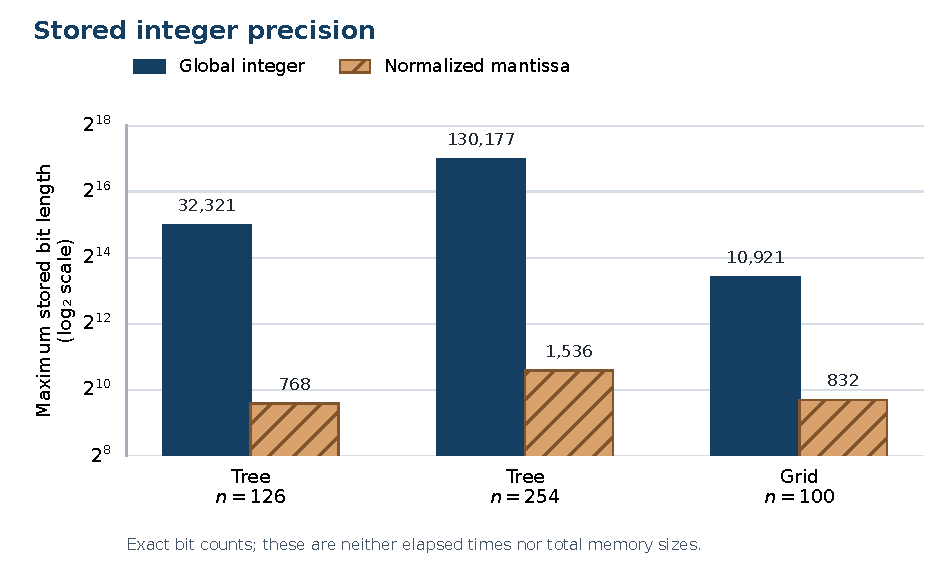
\includegraphics[width=0.92\linewidth]{figures/tensor_precision.pdf}
\caption{Retained scalar precision in the same exact tensor contraction,
with and without valuation normalization. The axis is logarithmic and the
labels give exact bit counts. This measures monomial-padding removal, not
an asymptotic running-time fit or a change in frontier width.}
\label{fig:tensor-precision}
\end{figure}

The ordering controls also matter. The certified tensor orders complete the
two large tree cases where ordinary-order integer tensors hit the state cap.
Conversely, every tensor mode hits the cap on the shuffled 64-crossing grid,
while faithful Potts completes. Thus the new backend adds a stronger exact
general bound and an alternative performance profile; it does not dominate
the existing backend on the supplied finite corpus.

\subsection{Cocycle seeds: exact objectives and genuine manifolds}

The cocycle data contain seven explicit product-solid-torus cases, a
one-vertex numerical limitation example, and two genuine finite knot
exteriors. The product construction triangulates $D^2\times S^1$ by
staircase tetrahedra. It starts with the primitive circle cocycle and adds
a large global vertex coboundary. Hence the huge initial weight represents
the same fixed primitive class; this deliberately isolates dependence on
binary height size.

% Generated by reproduce/make_research_tables.py; edit the generator, not this file.
\begin{table}[H]
\centering\footnotesize
\setlength{\tabcolsep}{3pt}
\renewcommand{\arraystretch}{1.12}
\begin{tabular*}{\linewidth}{@{\extracolsep{\fill}}rrrrrr@{}}
\toprule
$T$ & \shortstack{Height\\bits} & $\bits(D_0)$ & $D_\star$ & \shortstack{Optimizer\\(ms)} & \shortstack{Checker\\(ms)}\\
\midrule
9 & 1 & 2 & 3 & 0.812 & 0.125\\
9 & 20 & 23 & 3 & 0.657 & 0.111\\
9 & 260 & 263 & 3 & 1.035 & 0.134\\
9 & 4100 & 4103 & 3 & 1.163 & 0.128\\
24 & 20 & 25 & 3 & 3.599 & 0.250\\
48 & 20 & 26 & 3 & 15.221 & 0.498\\
96 & 20 & 27 & 3 & 46.796 & 0.954\\
\bottomrule
\end{tabular*}
\caption{All seven product-solid-torus cases. $T$ is the number of tetrahedra; $D_0$ and $D_\star$ are the initial and optimal numbers of normal discs. Height bits are measured from the supplied local heights, rather than inferred from a case-name parameter. Times are single recorded calls, not paired benchmark medians. Optimization includes its internal certificate check; the checker column measures an additional certificate and face-matching check. These cases verify binary-height handling and the fixed-family optimum; they do not establish an end-to-end recognition speedup.}
\label{tab:cocycle-times}
\end{table}


The largest-height nine-tetrahedron case starts with a disc count having
4,103 bits and returns a three-disc meridian seed. Its flow still takes
exactly nine augmentations. It therefore tests the absence of loops
proportional to numerical weight. The timings in this table are individual
recorded observations, not paired medians or a random-knot study. In the
one-vertex numerical case, the initial and optimized counts remain equal;
the optimizer correctly certifies that a common vertex shift changes no
span. No manifold is asserted for that arbitrary-height one-row example.

For a geometric test independent of the artificial large coboundaries, the
audit truncates two-tetrahedron ideal trefoil and figure-eight exteriors to
finite triangulations. Each has 56 tetrahedra and ten vertices. The existing
archive02 exact spanning-tree routine supplies a cocycle; rank one and a
coordinate gcd of one verify integral primitivity. The optimizer does not
choose a different homology class.

% Generated by reproduce/make_research_tables.py; edit the generator, not this file.
\begin{table}[H]
\centering\footnotesize
\setlength{\tabcolsep}{3pt}
\renewcommand{\arraystretch}{1.12}
\begin{tabular*}{\linewidth}{@{\extracolsep{\fill}}lrrrrrrr@{}}
\toprule
Knot exterior & $T$ & $|V|$ & $D_0$ & $D_\star$ & \shortstack{Optimizer\\(ms)} & $\chi$ & $b$\\
\midrule
Trefoil & 56 & 10 & 109 & 54 & 19.655 & -1 & 1\\
Figure-eight & 56 & 10 & 60 & 38 & 20.832 & -1 & 1\\
\bottomrule
\end{tabular*}
\caption{Two genuine finite knot exteriors obtained by truncating Regina's ideal examples. A primitive tree-gauge cocycle is optimized within its vertex-potential family. Regina independently verifies that each output is connected and orientable; $\chi$ and $b$ denote its Euler characteristic and boundary-component count. The single-call times include the triangulation adapter's seed construction and consistency checks, but exclude triangulation construction, cohomology preparation, and the independent Regina check. Disc-count optimality in this family does not assert genus minimality or incompressibility.}
\label{tab:cocycle-exteriors}
\end{table}


The disc counts fall from 109 to 54 and from 60 to 38. Regina independently
checks valid orientable finite manifolds and connected orientable surfaces
of Euler characteristic $-1$ with one boundary component. Exact gluings,
isomorphism signatures, cocycles, normal coordinates, and primal/dual
certificates are included in the JSON. Simplifying these exteriors first
produces one-vertex triangulations and removes this optimization freedom;
the choice to optimize the finite truncations is explicit.

Fifteen focused tests also compare small instances against exhaustive
primal searches and dual permutation oracles, exercise repeated vertices
and cancellation, reject corrupt certificates, handle 4,096-bit heights,
and check archive02 interoperability. The independently verified equality
of primal and dual objectives is the evidence of optimality. A decreased
disc count by itself is not evidence of faster hierarchy construction.

\subsection{Overlap measurements, controls, and unchanged corpus paths}

\begin{table}[H]
\centering\small
\begin{tabular}{@{}lrrrrr@{}}
\toprule
Family, $N=2^h$ & Old ms & A/A ms & Witness ms & Witness work & Nodes\\
\midrule
Prefix, $h=8$ & 174.971 & 161.297 & 0.551 & 708 & 64\\
Prefix, $h=32$ & LIMIT & LIMIT & 0.731 & 1,308 & 112\\
Prefix, $h=500$ & LIMIT & LIMIT & 5.220 & 13,008 & 1,048\\
Interior, $h=8$ & 201.398 & 159.737 & 0.503 & 962 & 76\\
Interior, $h=32$ & LIMIT & LIMIT & 1.239 & 1,898 & 148\\
Interior, $h=500$ & LIMIT & LIMIT & 8.100 & 20,150 & 1,552\\
Shared tail, $h=500$ & 7.012 & 5.772 & 6.916 & 12,939 & 1,042\\
Gain tradeoff & 0.240 & 0.231 & 0.190 & 488 & 43\\
\bottomrule
\end{tabular}
\caption{Five-round medians for complete local search and application.
The strict-majority family has the same final overlap and gain in each
successful arm. The gain-tradeoff row intentionally has different move
quality. LIMIT means exhaustion of two million charged work units.}
\label{tab:overlap-times}
\end{table}

On the $h=8$ prefix and interior cases, old charged work is respectively
245,591 and 319,306 units. The optional counts are 708 and 962. For larger
$h$, the old arms exceed the allowance, so no numerical speedup factor is
reported. The retained shared-tail control shows no convincing gain, as
predicted by the cyclic-factor analysis. In the no-majority $h=500$ control,
all arms exhaust in whole-donor search with zero witness-helper calls.

All 225 measured whole-knot queries retain identical certificate digests,
and none reaches the changed compressed LCS helper. The sums of medians for
fourteen smaller inputs are 140.334, 140.396, and 138.959 ms for old, A/A,
and optional arms. Gordian medians are 1.5253, 1.5104, and 1.4790 seconds.
These numbers support no knot-corpus speedup claim for the new helper.

The reachable Gordian residual produces the same first move, 142-move
certificate, and 4,280 allocated nodes in each arm. Charged work changes
only from 155,142 to 155,168. Its five-round medians, 69.55, 63.42, and
87.21 ms, fluctuate more than the small work difference would suggest and
show no stable improvement. The complete trace is supplied because it
validates the real certificate boundary, not because its timing favors the
new method.

\subsection{Maintained test inventory and the worker correction}

Final discovery contains 721 tests in 83 maintained modules. The recorded
validation covers this inventory through ordinary \code{unittest} module
runs, with Regina distribution 7.4.1 enabled and no skipped tests. Before
the worker repair, all 720 then-existing tests ran: 719 passed and the
unchanged large-input worker regression raised a timeout. That error
reproduced in isolation. It was a compatibility defect in partial-input
communication on the inspected Python 3.12.14 runtime, rather than evidence
of a mathematical failure in any of the three primitives.

Only \path{fastunknot/normal_surface.py} and its test module changed after
that comprehensive batch. The other 82 modules supply 712 passing tests;
the affected worker module subsequently passes all nine tests, including
one added cleanup regression. Thus the final coverage is
$712+9=721$ current tests. A further six-test public-integration rerun also
passes; those six belong to the retained 712 and are not counted twice.
The affected module is the only test module using the worker transport;
the cocycle adapter tests import Regina directly. No existing test's
deadline or expectation was relaxed. The complete accounting, final source
hashes and raw logs are in \path{validation/final-validation.json} and the
adjacent validation files.

An earlier single-process discovery attempt ended with exit code 1 after
14 passing lines, without a unittest summary or traceback. Its cause was
not established; the next test passed in isolation. This attempt is
preserved and classified as incomplete, separately from the comprehensive
module runs. We do not report a successful final single-process suite run.


The checks distinguish discovery from verification. Seed-certificate
verification runs without the flow solver. Group-certificate replay runs
without the producer. Tensor output is compared to both an independent
state-sum oracle and an external exact implementation. Resource tests ensure
that incomplete operations cannot publish a partial invariant or a false
decision. Those boundaries are more consequential than simply increasing
the number of test cases.

\subsection{Interpretation of the evidence}

The empirical conclusions are deliberately specific. The binary tensor
backend improves a proved repository asymptotic bound. Valuation normalization
removes measured arithmetic overhead within that backend. Cocycle flow
reduces a certified geometric objective on two actual knot exteriors and
handles huge binary heights without expansion. Threshold-first overlap
substantially accelerates a proved compressed stress family. None of these
observations demonstrates a quasi-polynomial growth law for complete
recognition, and the supplied negative controls identify concrete reasons
why such an inference would be invalid.

\addtocontents{toc}{\protect\newpage}
\section{Integration, certificate boundaries, and resource behavior}
\label{sec:integration}

The source patch keeps each optional experiment available through a supported
interface. The new production modules have no mandatory third-party Python
dependency. Regina is used for optional geometric checks and the existing
external fallback, not for either the tensor implementation or the cocycle
flow solver.

\subsection{Using the exact tensor backend}

From the \code{fast} directory, the standalone command computes a full
polynomial and reports its one-sided recognition consequence:
\par\noindent\begin{minipage}{\linewidth}
\begin{lstlisting}[language=bash]
python -B -m fastunknot jones examples/trefoil.json --backend tensor
python -B -m fastunknot jones examples/hard_unknot_8.json --backend tensor
\end{lstlisting}
\end{minipage}\par

The first input has a nonidentity polynomial; the second has identity and
the standalone Jones command is inconclusive about knot type. To use the
tensor stage within the full recognizer:
\par\noindent\begin{minipage}{\linewidth}
\begin{lstlisting}[language=bash]
python -B -m fastunknot recognize examples/hard_unknot_8.json \
  --jones-backend tensor
\end{lstlisting}
\end{minipage}\par

Other earlier stages may already decide this small input. Tests explicitly
disable those stages when checking that tensor identity continues to the
Khovanov fallback, and that a separately exhausted fallback returns
\status{UNKNOWN} rather than misusing Jones identity.

The low-level interface is:
\par\noindent\begin{minipage}{\linewidth}
\begin{lstlisting}[language=Python]
from fastunknot import Diagram
from fastunknot.tensor_jones import tensor_jones

diagram = Diagram.from_braid(3, [1, -2] * 5)
result = tensor_jones(
    diagram, certified=True, arithmetic="integer",
    max_states=4096, max_transitions=200000,
)
\end{lstlisting}
\end{minipage}\par

The result contains the exact full polynomial as signed hexadecimal integer
coefficients indexed by integral $t$-exponent, the chosen order and separator
certificate, crossing count, writhe, and measured resource counters. Hex
encoding avoids dependence on a runtime's decimal-digit conversion limit
for very large exact integers. Callers can select \code{"laurent"} for the
reference calculation or \code{"integer-global"} for the arithmetic
ablation. The latter intentionally preserves an inefficient monomial-shift
scheme for comparison.

The retained state and transition limits count mathematical work objects.
They do not independently cap the bytes occupied by a large integer.
Deadline callbacks are checked during preparation, state updates,
coefficient loops, and decoding. A running big-integer operation is not
preempted at an arbitrary machine instruction, so these are cooperative
allowances rather than hard real-time guarantees.

\subsection{Optimizing and checking a cocycle seed}

The numeric API accepts four global vertex IDs and four integral heights
per tetrahedron:
\par\noindent\begin{minipage}{\linewidth}
\begin{lstlisting}[language=Python]
from fastunknot.cocycle_seed import (
    minimize_disc_seed, check_seed_certificate,
)

certificate = minimize_disc_seed(vertices, heights)
checked = check_seed_certificate(vertices, heights, certificate)
assert checked["primal"] == checked["dual"]
\end{lstlisting}
\end{minipage}\par

It rejects malformed rows and nonintegral values. The checker recomputes
the potential-adjusted local gaps, disc counts, shared-vertex matching,
source and target permutations, and objective equality. It does not call
the optimizer or trust its reported statistics.

There are two geometric adapters. The face-pairing API validates reciprocal
gluings, local integer height transitions, and normal matching. The
triangulation-protocol API accepts a separately validated finite
triangulation and integral cocycle, including the archive02 object used in
the tests. The optimization theorem needs only numeric data; the topological
theorems additionally need a genuine compact orientable manifold,
coorientation, and the stated integral class conditions. No adapter silently
infers manifold validity from an optimal flow.

A normal-coordinate vector together with a primal/dual matching certifies
the restricted minimum-disc problem. It does not certify that the surface
is incompressible or that a subsequent hierarchy is essential. Those are
separate certificate types. The proposed Euler-characteristic positive test
in Section~\ref{sec:cocycle} would also require independently bound
knot-exterior provenance and peripheral data before it could decide an
input diagram.

\subsection{Enabling the overlap witness policy}

The new CLI flag enables its required compressed search and relator moves:
\par\noindent\begin{minipage}{\linewidth}
\begin{lstlisting}[language=bash]
python -B -m fastunknot recognize examples/hard_unknot_8.json \
  --group-overlap-witness --group-seconds 2
\end{lstlisting}
\end{minipage}\par

Python callers select the related flags explicitly:
\par\noindent\begin{minipage}{\linewidth}
\begin{lstlisting}[language=Python]
result = recognize(
    diagram,
    use_group=True,
    group_compressed_search=True,
    group_relators=True,
    group_overlap_witness=True,
)
\end{lstlisting}
\end{minipage}\par

The standalone compressed producer accepts
\code{relator\_moves=True, overlap\_witness=True}; the local helper accepts
\code{witness\_first=True}. Non-Boolean values and inconsistent option
combinations are rejected. The adaptive explicit-to-compressed policy is a
different interface and is not silently changed by this option.

Search still has the same resource semantics: a verified successful group
certificate proves the existing conclusion, while an unsuccessful or capped
search remains inconclusive. The first-witness policy may change a future
search trajectory, which is why it is not made the default. Neither
independent verifier needs to know which search policy discovered a move.

\subsection{Repairing large requests to the external normal-surface worker}

The maintained test inventory exposed a separate, reproducible compatibility
bug in the existing worker transport. The parent initially called
\code{communicate(payload, timeout=...)} and retried with no input after a
short timeout. In the tested Python 3.12.14 runtime, the communication code
retained its internal input buffer but registered writable stdin only when
the current call supplied a truthy input argument. A delayed reader with a
500-kilobyte request could therefore receive only the first pipeful, while
the parent waited until its three-second test allowance expired.

The repair gives one communication thread sole ownership of
\code{communicate(payload)}. The caller waits on a completion event in
bounded intervals, checking the existing local deadline and global
cancellation callback on the calling thread. Completion publishes either
the returned streams or the communication error. A worker pipe failure
remains inconclusive, while a caller's cancellation exception propagates.

Cleanup covers every operation after successful child creation, including
event construction, thread construction and startup. It kills a live
child, reaps it, joins a successfully started communicator, and then closes
the pipes. Independent review identified and closed a constructor-scope
gap before the final tests. The scope is the controlled direct-child
Regina worker; it is not a general supervisor for arbitrary grandchildren
retaining inherited pipes.

The existing delayed-reader regression now transmits and recovers all
500,000 input characters within its unchanged three-second allowance.
Existing cancellation and real-engine checks also pass. One additional
test injects communication and thread-setup failures, verifies child
reaping and closed pipes, checks that the payload is submitted once, and
confirms caller-thread polling. The final nine-test worker module passes
in 2.732 seconds, followed by six public-integration tests in 0.010 seconds.
The preserved diagnosis and logs are separate from the performance
benchmarks; this transport repair contributes no claimed mathematical
speedup.


This is an engineering correctness and performance repair, not a new
topological theorem. The external engine remains explicitly trusted for
its own topology operations. Digest validation, response schema checks,
decision semantics, and the complete built-in fallback remain in force.

\subsection{What an independent verifier does and does not establish}

\begin{table}[H]
\centering\small
\begin{tabularx}{\linewidth}{@{}P{0.22\linewidth}YY@{}}
\toprule
Evidence & Independent check & Conclusion\\
\midrule
Separator hierarchy & Graph partition, balance, order, cut width &
The stated width bound for that input and order.\\[3pt]
Full tensor polynomial & State-sum and Regina comparison in the audit &
Implementation agreement on tested inputs; the general exactness theorem
comes from Section~\ref{sec:tensor}.\\[3pt]
Seed potential and matching & Recomputed local spans and equal dual bound &
Global optimality within the vertex-potential family.\\[3pt]
Relator trace & Literal or compressed move-by-move replay &
The existing group certificate conclusion for the original diagram.\\[3pt]
External normal decision & Input digest, process status, schema, engine label &
A completed externally trusted decision, not independent replay of a
geometric hierarchy.\\
\bottomrule
\end{tabularx}
\caption{Trust boundaries retained by the integration. A consistency check
is not automatically a certificate of a stronger mathematical claim.}
\end{table}

All complete output claims refer to a validated input. An invalid planar
encoding, unmatched normal coordinates, an inexact division, or a malformed
certificate is a failed operation. A resource exhaustion is a different
outcome and remains inconclusive. Preserving this distinction is essential
when combining several exact and heuristic discovery stages in one
recognizer.

\section{What is still needed for quasi-polynomial recognition}
\label{sec:research}

The most useful next step is to make the missing global bounds explicit
enough to prove, refute, or measure. A vague expectation that every local
operation is fast is not an adequate complexity argument. In particular,
binary coordinates can encode exponentially many discs, a small grammar can
undergo exponentially many valid rewrites, and a small boundary alphabet
can carry a large algebraic object.

\subsection{A complete accounting identity}

Let $R$ be the number of processed search or hierarchy states, let $S_j$
be the complete binary encoding size of state $j$, and let $C_j$ be the
cost of generating, transforming, and checking it. If local operations have
a uniform polynomial bound $C_j\leq(S_j+N)^d$, then
\begin{equation}
 \operatorname{Time}(N)
 \leq\operatorname{preparation}(N)+
 R\left(N+\max_j S_j\right)^d.
 \label{eq:global-accounting}
\end{equation}
Thus both $R$ and the maximum represented size must be quasi-polynomial.
This elementary inequality is the central obligation that the three new
primitives do not yet discharge.

For the hierarchy route, the lexicographic reset accounting in
\cite[Section~9]{lackenby2026} gives at most $L(g+1)^L$ passes through a
step, where $L$ bounds hierarchy length and $g$ bounds relevant
pattern-complexities. Taking logarithms shows the precise requirement:
\begin{equation}
 \log L+L\log(g+1)\leq(\log(N+2))^{O(1)}
 \label{eq:reset-target}
\end{equation}
would suffice for the iteration part of a quasi-polynomial bound. A linear
bound on $L$ together with a polynomial bound on $g$ gives only an
$\exp(O(N\log N))$ reset estimate by this argument. Strict decrease of a
large integer potential proves termination, but is not the same as a small
number of decreases.

The refined hierarchy controls length through its initial handle complexity,
but this does not by itself supply \eqref{eq:reset-target}. A successful
program could either obtain much stronger simultaneous depth and complexity
bounds, or replace the lexicographic reset estimate with a better amortized
or memoized one. The latter may be more plausible than forcing every
decomposition to halve a topological quantity. In either case the actual
compressed cutting and attaching operations must satisfy the local cost
assumption in \eqref{eq:global-accounting}.

\subsection{A conditional composition theorem with explicit hypotheses}

The following statement is an accounting tool, not a theorem that the current
hierarchy or group search satisfies its hypotheses.

\begin{theorem}[Conditional quasi-polynomial composition]
Suppose a complete recognition procedure on an $N$-bit input can be organized
as a rooted search tree with the following properties, for fixed constants
$a,b,c,d,C$:
\begin{enumerate}
\item its depth is at most $C\log^a(N+2)$;
\item each node has at most $(N+2)^c$ children, including every necessary
branch of the complete procedure;
\item every node, attaching map, integer, and certificate needed locally
has total binary encoding size at most $\exp(C\log^b(N+2))$;
\item constructing a node, deciding its local actions, checking its
certificate, and verifying a leaf take time at most the $d$th power of its
encoding size plus $N$.
\end{enumerate}
Then the complete procedure has quasi-polynomial bit time and can be
executed in quasi-polynomial space by depth-first traversal.
\label{thm:conditional-qp}
\end{theorem}
\begin{proof}
The number of nodes is bounded by a geometric sum with largest term
\[
 ((N+2)^c)^{C\log^a(N+2)}
 =\exp(O(\log^{a+1}(N+2))).
\]
The per-node cost is $\exp(O(\log^b(N+2)))$ times a polynomial factor in
$N$. Multiplying gives
$\exp(O(\log^{\max(a+1,b,1)}(N+2)))$. The active path has
polylogarithmic length and each stored state has the stated bound; the local
workspace is bounded by the local running time. This gives the space
conclusion. Completeness is an explicit hypothesis; it is not
obtained from this counting argument.
\end{proof}

Another route replaces depth and branching by a proved quasi-polynomial
bound on the number of distinct canonical states and a rule that expands
each at most once. That requires a canonical representation preserving all
attaching and boundary-pattern data. Equal coarse statistics or isomorphic
unlabelled incidence graphs are not automatically equivalent states for a
future geometric continuation.

For a width-based route, $w=\log^{O(1)}N$ makes the binary tensor primitive
quasi-polynomial immediately. Planarity alone only supplies $w=O(\sqrt n)$.
Moreover, exact Jones identity still requires an independent completion
route in this implementation. A width theorem and a complete treatment of
identity cases would therefore both be needed before that observation became
a recognition theorem.

\subsection{Safe portfolio accounting}

The measurements suggest a practical improvement that already has a simple
complexity proof: run faithful Potts for a polynomially bounded amount of
whole-query work, and if it does not finish, run the certified binary tensor
algorithm from the validated diagram. The first arm is often much cheaper
on the current corpus. The second supplies the better universal bound.

\begin{proposition}[A bounded prelude preserves a fallback bound]
If an exact prelude costs at most $p(N)$ bit operations and returns either
a checked answer or an inconclusive result, while an exact complete fallback
costs at most $F(N)$, sequential composition costs at most $p(N)+F(N)$ and
is exact. In particular, a polynomially bounded faithful-Potts prelude
preserves the binary tensor full-Jones bound.
\end{proposition}
\begin{proof}
The prelude either supplies a checked answer within its budget or consumes
at most $p(N)$ before the fallback starts. The fallback receives the original
validated problem. Its cost and correctness then apply independently of the
failed prelude. Adding the bounds proves the claim.
\end{proof}

The budget must include preparation, all attempted shadings or orders,
coefficient arithmetic, and normalization, not just one inner transition
counter. In this implementation those operations have polynomial bit bounds
per represented work object, so a proved polynomial transition and state
budget can support such a prelude. The portfolio itself is proposed, not
part of the frozen patch.

There is an analogous constraint on an eventual quasi-polynomial recognizer:
it cannot always insist on finishing an uncapped $2^{O(\sqrt n)}$ invariant
first and then claim a quasi-polynomial total from a later stage. Such an
invariant must have its own quasi-polynomial allowance, be skipped, or be
proved cheaper on the relevant branch. Optional heuristics are compatible
with a good worst-case theorem when their discarded work is explicitly
bounded.

\subsection{Priority I: complete compressed geometry}

\begin{question}[Exact cutting with complete attaching data]
Can a cut along a binary normal surface be computed and independently
verified in time polynomial in the triangulation size, coordinate bit
length, and size of the compressed output, without enumerating individual
discs or parallel product regions?
\end{question}

This is the most consequential implementation target for the hierarchy
route. A useful representation must retain oriented attaching intervals,
boundary patterns, component identities, and maps back to the original
manifold. Merely recording multiplicities of local normal disc types does
not say how the new boundary pieces are paired. A benchmark should therefore
include exponentially large parallel families with a fixed number of local
types, and compare the compressed result with a literal cut on all feasible
small members. The pass condition is equality of reconstructed attaching
maps and certificate replay, together with output-size and bit-cost bounds.

\begin{question}[Certified parallelity reduction]
Can all relevant product or parallelity regions be recognized and collapsed
using compressed interval data, with a certificate of the resulting handle
structure and inherited boundary pattern?
\end{question}

This would connect the implementation to the refined hierarchy's depth
control. It must include exceptional or non-disk bundle bases and their
vertical boundaries, rather than assuming every repeated local block is a
trivial product. A concrete first milestone is an exact list of permitted
local quotient operations, each with a reconstruction certificate and
explicit effect on the chosen complexity measure. The benefit should be
measured in compressed handle count and subsequent reset work, not only in
the number of expanded tetrahedra avoided.

\begin{question}[Normal curves after a compressed cut]
Can boundary intersection, isotopy, and normalization operations be made
polynomial in all representation parameters actually produced by cutting?
\end{question}

Lackenby's fast curve algorithms provide suitable starting primitives
\cite{lackenbycurves2026}. Their hypotheses and parameters must be preserved
at the adapter boundary. In particular, standard-curve normalization depends
on its simplification number as well as triangulation size and logarithmic
weight. Controlling only binary multiplicities is therefore insufficient if
the cut creates many independently paired arc pieces. The next artifact
should expose that pairing count or simplification number as a measured and
proved state-size parameter, with literal small-instance comparison.

\begin{question}[Independent geometric decision certificates]
Can a successful hierarchy, crushing sequence, or meridian disk be exported
from discovery and replayed by a small exact checker bound to the original
diagram and its peripheral data?
\end{question}

The cocycle matching is a model for this boundary: the solver proposes a
small certificate and a separate routine checks the claimed objective.
Geometry needs richer witnesses, including the validity of the exterior,
essential boundary slopes, and the admissibility of each operation. A first
positive milestone is the Euler-characteristic disk test proved in
Section~\ref{sec:cocycle}. Its implementation should not mistake a rank-one
manifold for the input knot exterior or use a disk with inessential boundary
as an unknot certificate.

\subsection{Priority II: a global descent or reset theorem}

\begin{question}[Reset accounting stronger than lexicographic termination]
Is there an amortized potential, persistent-prefix reuse theorem, or
canonical-state bound that replaces $L(g+1)^L$ by a quasi-polynomial bound
on actual reconstruction work?
\end{question}

An informative experiment must record why a prefix is discarded, what data
remain reusable, and how much later work is repeated. Counting only successful
decompositions hides the potentially dominant cost. A candidate theorem
should specify an injection from reset events into a bounded family of
combinatorial objects or prove a multiplicative decrease after a bounded
batch of events. If neither can be shown, an explicit family with repeated
near-identical resets would be a valuable negative result.

\begin{question}[State size under repeated cutting and simplification]
Can the complete compressed state remain quasi-polynomial in the original
diagram size throughout every necessary branch?
\end{question}

The word ``complete'' includes coefficient bits, interval endpoints,
pairings, boundary-pattern labels, and certificate history. A fixed local
alphabet of handle types is helpful but does not bound the number of copies
or distinct attaching patterns. A proposed invariant should have a bound
under each primitive and under composition; an individual output-sensitive
algorithm alone does not prevent its outputs from growing too quickly.
Recording both peak size and cumulative newly created data will distinguish
reusable DAG sharing from repeated copying.

\begin{question}[Algebraic summaries beyond the Jones state space]
Can a complete detecting invariant or geometric boundary condition be
represented at polylogarithmic interfaces with quasi-polynomial total
algebraic multiplicity and update cost?
\end{question}

Replacing Bell partitions by binary states solves a specific invariant
calculation. It cannot simply be transferred to Khovanov complexes: the
number of boundary labels does not bound chain-group multiplicities,
differential data, or the work needed to perform exact cancellation and
rank decisions. Even with one boundary label, an abstract chain object can
carry arbitrarily many summands. A viable stronger summary needs an exact
composition theorem controlling those data, with proof that the final
decision is complete. Small widths on special diagram classes should be
studied separately from claims about arbitrary planar diagrams.

\subsection{Priority III: improving the new primitives}

\begin{question}[Weighted and class-aware cocycle optimization]
Can the certified flow objective be extended to local geometric costs that
predict hierarchy work, and can a bounded set of cohomology classes be
searched without losing a global bit bound?
\end{question}

Positive integral tetrahedron weights preserve the network formulation, but
require a flow algorithm polynomial in binary capacities. Minimizing genus
or pattern-complexity is not obtained simply by renaming the disc-count
objective. Varying the cohomology class also leaves the current potential
family and may reintroduce an integer search problem. A useful first result
would state exactly which weighted local objectives remain convex network
spans, and compare their certified optima with measured cut or reset costs
on genuine knot exteriors. The rank-one primitive case is a natural initial
target because its class choices are controlled.

\begin{question}[When does additional vertex freedom justify its cost?]
Can truncation or subdivision be chosen by a certified benefit/cost rule
that improves seed construction or downstream geometry on difficult inputs?
\end{question}

The finite-exterior examples show useful freedom with ten vertices and none
after one-vertex simplification. More vertices do not automatically help:
they increase the flow and geometric state, and disc count changes with the
triangulation. A fair comparison should report the number of tetrahedra,
bits, normal discs, Euler characteristic, and actual downstream work. For
known pure gauge changes on a fixed triangulation, the certificate-transport
proposition avoids solving the flow again. Retriangulation requires a
separate transport theorem and cannot use that formula without proof.

\begin{question}[Smaller tensor work with the same certified bound]
Can order selection, outer-face selection, and a bounded faithful prelude
reduce actual state and arithmetic costs while preserving the universal
square-root bound?
\end{question}

The existing certificate allows heuristic orders to compete with a guaranteed
one. A cost model incorporating actual state multiplicity and mantissa bits
may predict runtime better than frontier width alone. Any order-search
budget must be charged. An especially useful negative deduction follows
from Proposition~\ref{prop:gauge}: changing only a same-outer bend gauge
cannot reduce normalized mantissas or their bit lengths for a fixed order.
Optimizing that gauge solely to shrink integer precision would be wasted
effort. Changing the outer face is a different operation and can be tested
explicitly, while retaining the complete turning proof. Sharper bounds on
formal coefficient span also remain a mathematical question, rather than
an assumed consequence of gauge covariance.

\begin{question}[Witness quality and the next compressed bottleneck]
Can a budgeted overlap scheduler obtain useful gain guarantees, while
rejecting impossible whole-donor queries before they consume the allowance?
\end{question}

The present first-witness gain ratio tends to zero on a proved family, so
an unconditional approximation theorem for this exact policy is unavailable.
A modified policy might retain several cheap witnesses, increase a threshold
geometrically, or optimize gain only within a controlled collection of
periodic alignments. Each proposal needs a clear extra-work bound and a
counterexample search. Independently, the pair $(ab)^N,(aabb)^N$ calls for
a cheap exact incompatibility summary of run lengths or periodic defects
at the earlier whole-donor stage. The relevant parameter may be defect count
in addition to grammar size and length bit size.

\begin{question}[From local group moves to complete bounded discovery]
For presentations arising from actual knot diagrams, can one prove a
quasi-polynomial bound on necessary moves, grammar growth, and certificate
size for a complete discovery strategy?
\end{question}

This is substantially harder than a polynomial local word theorem. A strict
decrease of expanded relator length may still allow exponentially many
unit decreases. Strong compression does not itself make the greedy move
set complete. Research should distinguish arbitrary synthetic presentations
from residuals reachable by verified transformations of Wirtinger
presentations. The next benchmark target is a collection of actual knot
residuals above the explicit bridge cap that genuinely exercise the new
partial-overlap stage, with independently replayed final certificates and
all preceding-stage work included.

\subsection{Milestones and decision criteria}

The priorities above can be organized into three reviewable releases.
The first should implement a capped full-Jones portfolio, seed-certificate
transport, and a peripheral-data-bound positive disk checker. Success means
unchanged exact outputs, independent certificate replay, and a documented
improvement on inputs that exercise the changed path.

The second should deliver compressed cutting and normal-curve adapters with
explicit output-size bounds, including product-region and boundary pairing
data. Success means agreement with literal topology on small cases and
polynomial dependence on binary weights on large structured families, with
no hidden disc expansion. If some family forces excessive pairing growth,
that obstruction should be stated before extending the hierarchy code.

The third should address \eqref{eq:reset-target} and
\eqref{eq:global-accounting}: prove an amortized reset or canonical-state
bound for a complete strategy, or construct a rigorous family showing that
the proposed strategy cannot satisfy it. A general quasi-polynomial claim
should be made only when the completeness theorem, state-size invariant,
primitive bit bounds, and total-work accounting all refer to the same
implemented or fully specified algorithm.

The work in this package makes the next stage concrete. It provides exact
primitives whose guarantees can be composed when the missing global
structure is available, and it identifies several attractive shortcuts
that fail under direct mathematical or experimental scrutiny.

\appendix
\section{Reproducibility and repository integration}
\label{app:reproduce}

\subsection{Package map}

The accompanying archive is organized as follows. Relative paths are from
the archive's top-level directory.
\begin{longtable}{@{}P{0.38\linewidth}P{0.58\linewidth}@{}}
\toprule
Path & Purpose\\
\midrule
\endhead
\path{article/unknot_certified_primitives.tex} & Main editable article;
section inputs, bibliography, generated tables, and vector figure are beside it.\\[4pt]
\path{article/unknot_certified_primitives.pdf} & Compiled and visually checked
article.\\[4pt]
\path{article/build.sh} & Rebuilds the article with PDFLaTeX through latexmk.\\[4pt]
\path{integration/changes.patch} & Repository-relative source patch against
the pinned baseline.\\[4pt]
\path{integration/tree/} & A runnable source snapshot preserving
\path{Topology/UnknotRecognition/} and the required reference packages.\\[4pt]
\path{integration/manifest.json} & SHA-256 hashes, changed-file inventory,
and baseline identity.\\[4pt]
\path{integration/patch-validation.json} & Temporary-index apply check and
byte-for-byte reconstruction of every changed file.\\[4pt]
\path{results/} & Full raw exact outputs, timing samples, table values,
completion status, and independent audits.\\[4pt]
\path{results/checkpoints/} & Earlier tensor arithmetic measurements,
explicitly distinguished from the final six-arm comparison.\\[4pt]
\path{certificates/} & Independently replayable original-diagram Gordian
certificate used by the overlap audit.\\[4pt]
\path{reproduce/} & Test runner, independent Regina audit, table/figure
generator, assembly helper, and detailed reproduction instructions.\\[4pt]
\path{validation/} & Unedited test outputs, final coverage composition,
worker-regression diagnosis, independent reviews, and article build/QA record.\\[4pt]
\path{provenance/} & Mathematical audit notes and primary-source metadata.\\
\bottomrule
\end{longtable}

The source snapshot contains the maintained \code{fast} code, tests,
fixtures, and reference packages from reports 02, 24, 26, and 28. It does
not duplicate the entire historical repository or bundle the external
Regina binary. Relevant existing licenses and package metadata are retained.
The final source patch modifies or adds eighteen files. It is accompanied
by a full snapshot so that mathematical review is not dependent on reading
a diff alone.

\subsection{Applying and checking the patch}

At the specified baseline checkout, first inspect the change summary and
perform the ordinary Git apply check:
\par\noindent\begin{minipage}{\linewidth}
\begin{lstlisting}[language=bash]
git rev-parse HEAD
git apply --check /path/to/package/integration/changes.patch
git apply /path/to/package/integration/changes.patch
\end{lstlisting}
\end{minipage}\par

The recorded baseline is
\begin{center}\small\baseline\end{center}
If integrating after later repository work, review any conflicts against
that baseline instead of assuming the patch's context still matches.
The delivered package was checked in a separate temporary index: the patch
applied and every reconstructed changed file matched the snapshot by hash.
This did not modify the checkout's real index or create a remote commit.

The article can be placed with the repository's research reports and linked
from the synthesis documents during integration. It is self-contained and
does not require historical article fragments to compile. Its proofs make
clear which algorithms are newly implemented, which bounds were already
known, and which routes remain conditional.

\subsection{Tests and independent audits}

From the source snapshot or integrated checkout's \code{fast} directory:
\par\noindent\begin{minipage}{\linewidth}
\begin{lstlisting}[language=bash]
python -B -m unittest discover -s tests -v
python -B audit_tensor_jones.py \
  --output results/tensor_jones_audit_local.json
python -B benchmark_tensor_jones.py --rounds 7 --seconds 2 \
  --output results/tensor_jones_local.json
python -B benchmark_cocycle_seed.py --regina \
  --output results/cocycle_seed_local.json
python -B benchmark_overlap_witness.py \
  --output results/overlap_witness_local.json
\end{lstlisting}
\end{minipage}\par

The optional Regina version used here is 7.4.1. Without it, the base modules
remain usable but independent geometric tests are not the same validation
run. The module-by-module test runner documents an alternative complete
inventory route and the exact final coverage composition.

The overlap historical comparison reads the archived helper from Git at the
pinned revision. It therefore requires that Git object, normally supplied by
the target repository checkout. The standalone current-code snapshot suffices
for its tests and ordinary use, but does not recreate absent Git history.
The README records this prerequisite explicitly.

The independent Regina audit runs from the package directory:
\par\noindent\begin{minipage}{\linewidth}
\begin{lstlisting}[language=bash]
python -B reproduce/audit_regina_jones.py \
  --fast-dir /path/to/ProveIt/Topology/UnknotRecognition/fast \
  --output results/regina_jones_local.json
\end{lstlisting}
\end{minipage}\par

An optional \code{--regina-path} supplies a separate dependency installation.
The audit validates variable conventions and compares whole coefficient
maps. It does not use a polynomial digest as a substitute for equality.

\subsection{Rebuilding the article and tables}

The main document uses standard TeX Live packages and no shell-escape
extension. Tables and the figure can be regenerated from archived JSON:
\par\noindent\begin{minipage}{\linewidth}
\begin{lstlisting}[language=bash]
python -B reproduce/make_research_tables.py
sh article/build.sh
\end{lstlisting}
\end{minipage}\par

The figure generator uses Matplotlib; \code{--tables-only} avoids that
dependency when the supplied vector figure is retained. Table generation
checks the median calculations against individual samples and does not
rerun a benchmark. Earlier checkpoint timings are not mixed into the final
table.

The PDF has been rendered to page images and inspected for clipping,
unreadable tables, malformed mathematics, and unintended blank pages.
Build diagnostics and the page-level review record are retained under
\path{validation/}. Auxiliary TeX build products are unnecessary for source
reproduction, apart from the supplied bibliography source and generated
figure assets.

\subsection{Limitations of the research record}

This is a research continuation prepared with AI assistance, with separate
mathematical, algorithmic, and literature audit passes. Those checks are not
external peer review, and the mathematical proofs have not been formalized
in a proof assistant. The article supplies enough definitions, proofs,
counterexamples, and exact artifacts for further scrutiny rather than asking
the reader to accept a performance claim from an informal summary.

The initial incomplete test process and the reproduced pre-fix worker failure
are retained separately from successful final coverage. Timings are from a
single recorded environment. The current knot corpus does not exercise the
new compressed partial-overlap path during ordinary complete queries.
The normal-seed objective does not certify incompressibility, and the tensor
bound concerns full Jones computation. A general quasi-polynomial bound
for the maintained complete recognizer remains a goal of the research
program, not a deliverable claimed by this package.

\bibliographystyle{plain}
\bibliography{references}
\end{document}
